% !TeX encoding = UTF-8 Unicode
\documentclass[a4paper,12pt]{article}
\usepackage[english]{babel}
\usepackage[english]{isodate}
\usepackage{graphicx}
\usepackage{hyperref}
\usepackage{centernot}
\usepackage{xfrac}
\usepackage{mathtools}
\usepackage{enumitem}
\usepackage{fancyhdr}
\usepackage{lastpage}
\usepackage{xcolor}
\usepackage{changepage}
\usepackage{amsthm}
\usepackage{amsfonts}
\usepackage{amsmath}
\usepackage{amssymb}
\usepackage{soul}
\usepackage{float}
\usepackage{centernot}
\usepackage{tcolorbox}
\usepackage{titling}
\usepackage{caption}
\usepackage{subcaption}
\usepackage{etoolbox}
\usepackage{listings}
\usepackage{biblatex}
\usepackage{csquotes}
\usepackage{titlesec}
\usepackage{tikz}
\usetikzlibrary{trees}

\addbibresource{bibliography.bib}

\patchcmd{\section}{\bfseries}{\bfseries\boldmath }{}{}
\patchcmd{\subsection}{\bfseries}{\bfseries\boldmath }{}{}
\patchcmd{\subsubsection}{\bfseries}{\bfseries\boldmath }{}{}

\hypersetup{
  colorlinks=True,
  urlcolor=blue,
  citecolor=red,
  menucolor=black,
}

\renewcommand{\UrlFont}{\ttfamily\footnotesize}

\lstdefinelanguage{futhark}
{
  % list of keywords
  morekeywords={
  do,
  else,
  for,
  if,
  in,
  include,
  let,
  loop,
  then,
  type,
  val,
  while,
  with,
  module,
  def,
  entry,
  local,
  open,
  import,
  assert,
  match,
  case,
  },
  sensitive=true, % Keywords are case sensitive.
  morecomment=[l]{--}, % l is for line comment.
  morestring=[b]" % Strings are enclosed in double quotes.
}


\lstset{
  language=futhark,
  showspaces=false,
  showstringspaces=false,
  mathescape=true,
  aboveskip=0pt,
  belowskip=6pt,
  numberstyle=\tiny,
  numbers=left, 
  firstnumber=1,
  numberfirstline=true,
  tabsize=4,
  breaklines=true,
}

\newcommand\LAST{\text{LAST}}
\newcommand\defiff{\mathrel{\stackrel{\makebox[0pt]{\mbox{\normalfont\tiny def}}}{\iff}}}
\newcommand\defeq{\mathrel{\stackrel{\makebox[0pt]{\mbox{\normalfont\tiny def}}}{=}}}
\newcommand\concat{\: \mathrlap{+} \: +}
\newcommand\map{\textbf{map}\ }
\newcommand\reduce{\textbf{reduce}\ }
\theoremstyle{definition}
\newtheorem{definition}{Definition}[section]
\newtheorem{proposition}{Proposition}[section]
\newtheorem{corollary}{Corollary}[section]
\newtheorem*{remark}{Remark}
\newtheorem{lemma}{Lemma}[section]
\newtheorem{theorem}{Theorem}
\newtheorem{algorithm}{Algorithm}[section]
\newtheorem{example}{Example}[section]
\newtheorem{conjecture}{Conjecture}[section]
\DeclareMathOperator{\sign}{sign}
\newcommand\doubleplus{+\kern-1.3ex+\kern0.8ex}
\newcommand\mdoubleplus{\ensuremath{\mathbin{+\mkern-10mu+}}}

\newcommand{\id}[1]{\ensuremath{\mathit{#1}}}
\newcommand{\kw}[1]{\ensuremath{\mathtt{#1}}}
\newcommand{\Let}{\kw{let}}
\newcommand{\In}{\kw{in}}
\newcommand{\If}{\kw{if}}
\newcommand{\Then}{\kw{then}}
\newcommand{\Else}{\kw{else}}
\newcommand{\Filter}{\kw{filter}}
\newcommand{\Or}{\kw{or}}
\newcommand{\Groupby}{\kw{groupby}}
\newcommand{\Partition}{\kw{partition}}
\newcommand{\Scatter}{\kw{scatter}}
\newcommand{\Hist}{\kw{hist}}
\newcommand{\Map}{\kw{map}}
\newcommand{\Sum}{\kw{sum}}
\newcommand{\Mod}{\kw{mod}}
\newcommand{\Fst}{\kw{fst}}
\newcommand{\Snd}{\kw{snd}}
\newcommand{\Presum}{\kw{presum}}
\newcommand{\True}{\kw{true}}
\newcommand{\False}{\kw{false}}
\newcommand{\Sort}{\kw{sort}}
\newcommand{\Segor}{\kw{segor}}
\newcommand{\Hash}{\kw{hash}}
\newcommand{\Random}{\kw{random}}
\newcommand{\Iota}{\kw{iota}}
\newcommand{\Unzip}{\kw{unzip}}
\newcommand{\Unit}{\mathbf{unit}}
\newcommand{\Int}{\mathbf{int}}
\newcommand{\Bool}{\mathbf{bool}}
\newcommand{\Def}{\kw{def}}
\newcommand{\Rep}{\kw{rep}}
\newcommand{\Zip}{\kw{zip}}

\fancyhf{}
\setlength{\headheight}{14.49998pt}
\pretitle{\vspace{-120pt}\begin{center}}
\posttitle{\par\end{center}\vspace{-80pt}}
\fancyhead[C]{}
\fancyfoot[R]{Page \thepage \hspace{1pt} of \pageref{LastPage}}
\pagestyle{fancy}
\fancypagestyle{firstpage}{%
  \fancyhf{}
  \renewcommand{\headrulewidth}{0pt}
  \fancyfoot[R]{Page \thepage \hspace{1pt} of \pageref{LastPage}}
}
\title{
  {\Large \textsc{University of Copenhagen}} \\[5pt]
  {\large Data-Parallel Union-Find} \\[10pt]
  Author: William Henrich Due \\[0pt]
  Advisor: Troels Henriksen \\[0pt]
  Submitted: 25th of January, 2026.
}
\author{}
\date{}

\begin{document}
\maketitle
\thispagestyle{firstpage}

\section{Introduction}
This is a thesis preparation project about data-parallel union-find structure
well suited for a functional array language \cite{vanBalen2025comparing}. The
project is about the theory, implementation and usage of the structure. The
union-find structure is structure which allows for maintaining equivalences
between elements. Union-find operate on single elements but the data-parallel
variant operates on multiple elements, in this project the structure will have
the following operations.
\begin{itemize}
  \item \texttt{create}: Creating an union-find structure of $n$ elements.
  \item \texttt{union}: An input array of tuple pairs of elements will be
  unified and is therefore said to be ``equivalent''.
  \item \texttt{find}: An input array of elements where a single unique
  representative of the equivalence class is returned for every element.
\end{itemize}
Three different data-parallel union-find structures will be presented, a
union-find structure without any heurestics, a union-find structure using union
by rank and union-find structure using union by size. These structures are
implemented in the parallel functional array language Futhark and the
implementations are tested and benchmarked. In the end these implementations are
used in a region labeling example and type checking example.

\section{Theory}
This section will derive the theoretical foundation for a data-parallel
union-find. The theory is based on set theory and graph theory.
\subsection{Forests}
To be able to define a union-find structure we first need to define some basic
graph theory, specifically in relation to forests. The graphs used are directed
graphs $G = (V, E)$ where $V$ is a set of vertices and $E \subseteq V \times V$
is a set of directed edges. Initially we need a definition of what it means for
a vertex $u \in V$ to be reachable from vertex $v \in V$ meaning there is a path
from $u$ to $v$.

\begin{definition}[Reachability]
  A veterx $v \in V$ is \emph{reachable} from a vertex $u \in V$ in a directed
  graph $G = (V, E)$ if there exists a sequence of directed edges $e_1, e_2,
  \ldots, e_m \in E$ where $m \geq 1$ and $e_i = (v_{i-1}, v_i)$ for $1 \leq i
  \leq m$, such that $v_0 = u$ and $v_m = v$. We denote this by $u \leadsto_G v$
  and may write $u \leadsto v$ if it is clear what graph is refered to.
\end{definition}
\noindent One of the first properties of reachability is it is neither
\text{reflexive} nor \textit{irreflexive}. The reason for chosing such a
definition is that the definition of an cycle in a directed graph becomes
simply.
\begin{definition}[Cycle]
  A cycle in a directed graph $G = (V, E)$ has a cycle if there exists a $v \in
  V$ such that $v \leadsto v$.
\end{definition}
\noindent With this definition of cycles a forest can be defined as following:
\begin{definition}[Forest]
  A forest is a directed graph $F = (V, E)$ where $V$ is a set of vertices and $E
  \subseteq V \times V$ is a set of directed edges such that:
  \begin{enumerate}
    \item There are no cycles $v \centernot\leadsto v$ for all $v \in V$, and
    \item each vertex has at most one parent i.e. for all $(u, v_1), (u, v_2)
    \in E$ it holds that $v_1 = v_2$.
  \end{enumerate}
\end{definition}
\noindent With the definition of a forest we can now define roots in a forest.
\begin{definition}[Root]
  A vertex $v \in V$ in a forest $F = (V, E)$ is a root if it has no parent.
  This is defined as the predicate:
  \begin{align*}
    \mathcal{R}_F(v) : v \centernot\leadsto u \text{ for all } u \in V
  \end{align*}
\end{definition}
\noindent Using the definition of a root we can now define a tree as a special
case of a forest.
\begin{definition}[Tree]
  A tree is a forest $T = (V, E)$ where there exists a unique root $r \in V$
  such that $v \leadsto r$ for all $v \in V\backslash
  \{r\}$.
\end{definition}
\noindent Futhermore we will now work towards seeing a forest as a collection of
trees. To do this we first need to establish how many roots a forest has.
\begin{proposition}[Forest Root Count]\label{prop:forest-root-count}
    A forest $F = (V, E)$ where $|V| = n$ and $|E| = n - k$ has $k$ roots.
\end{proposition}

\begin{proof}
    Let $F = (V, E)$ be a forest where $|V| = n$ and $|E| = n - k$. By the
    second property of a forest then $n - k$ vertices must have a parent. Since
    there are $n$ vertices in total it follows that there are exactly $k$
    vertices $r_1, r_2, \ldots, r_k \in V$ that has no parent. Hence there are
    exactly $k$ roots in $F$.
\end{proof}
\noindent Knowing how many roots a forest has does not finish the picture of how
a forest is a collection of trees. We also need to show that each vertex also
has a path to a root.
\begin{proposition}[Root Path Exist]\label{prop:roots-path-exist} In a forest $F
  = (V, E)$ for each element $v \in V$ then there exists a root $r \in V$ such
  that $\mathcal{R}_F(r)$ and either $v \leadsto r$ or $v = r$.
\end{proposition}

\begin{proof}
  Let $F = (V, E)$ be a forest and $v \in V$ be an arbitrary element in $V$. By
  proposition \ref{prop:forest-root-count} there exists at least one root $r \in
  V$ such that $\mathcal{R}_F(r)$. This can be shown by structural induction on
  a vertex $v \in V$ that either $v = r$ or $(v, p) \in E$ such that $p \leadsto
  r$.
  \begin{itemize}
    \item If $(v, p) \notin E$ then $v \centernot\leadsto u \text{ for all } u
    \in V$ so $v = r$ and $\mathcal{R}_F(r)$.
    \item If $(v, p) \in E$ then by induction hypothesis $p \leadsto r$ such
    that $r \in V$ and $\mathcal{R}_F(r)$. It follows that since $v \leadsto p
    \leadsto r$ so $v \leadsto r$.
  \end{itemize}
\end{proof}
\noindent Lastly we can finish the picture of a forest being a collection of
trees by showing that the path from a vertex to a root is unique. So that there
is only one tree for each vertex in the forest.
\begin{proposition}[Unique Path]\label{prop:unique-path}
  Let $F = (V, E)$ be a forest and $v, u \in V$. If $v \leadsto u$ then the path
  from $v$ to $u$ is unique.
\end{proposition}
\begin{proof}
  Let $F = (V, E)$ be a forest, $v, u \in V$ and $v \leadsto u$. Since every
  vertex has at most one parent by the second property of a forest it follows
  that there is only one out going edge from each vertex in the path from $v$ to
  $u$. Hence the path from $v$ to $u$ is unique.
\end{proof}

\subsection{Union-Find Structure}
Using the definition of a forest we can now define a union-find structure, the
way it will represented is as a forest. Here the forest represents an
equivalence on $V$ where each tree in the forest represents an equivalence
class.
\begin{definition}[Union-Find Structure]
  A union-find structure is a forest $F = (V, E)$.
\end{definition}
\noindent The way this equivalence relation is defined is by the representative
of each element in the forest. The representative of a vertex is found by
traversing the edges in the forest until a root is found. Using the notion of a
root we can now define the representative of an element in a forest.
\begin{definition}[Representative]
  The representative of an element $v \in V$ in a forest $F = (V, E)$ is the
  root $r \in V$ such that there is a path from $v$ to $r$. This is defined as
  the function:
  \begin{align*}
    \rho_F(v) := r \text{ where } r \in V \text{ such that } \mathcal{R}_F(r) \land (v \leadsto r \lor v = r)
  \end{align*}
\end{definition}
\noindent With the notion of a representative it is possible to define the set
of vertices in the same tree in a forest.
\begin{definition}[Tree Set]
  The set of vertices of the same tree $\mathcal{E}_F(v)$ in a
  forest $F = (V, E)$ is defined as:
  \begin{align*}
    \mathcal{E}_F(v) := \{u : u \in V \text{ where } \rho_F(u) = \rho_F(v)\}
  \end{align*}
\end{definition}
\noindent The notion of equivalence classes can now be formalized using the
definition of a partition. This will be needed to show properties of the
union-find structure.
\begin{definition}[Partition]\label{def:partition}
  The set $P \subseteq \mathbb{P}(S)$ is a partition of a set $S$ if:
  \begin{enumerate}
    \item $a \neq \emptyset$ for all $a \in P$
    \item $a \cap b = \emptyset$ for all $a, b \in P$ where $a
    \neq b$
    \item $\bigcup_{a \in P} a = S$
  \end{enumerate}
  We say that $P$ is a partition of $S$ and $P$ forms an equivalence relation on
  $S$ where each $a \in P$ is an equivalence class.
\end{definition}
\noindent Using the definition of a partition we can now show that a forest is a
partition of its vertices based on the tree sets.
\begin{proposition}[Forest Partition]\label{prop:forest-partition}
  A forest $F = (V, E)$ is a partition of $V$ for the following set:
  \begin{align*}
    \{\mathcal{E}_F(v) : v \in V\}
  \end{align*}
\end{proposition}

\begin{proof}
  Let $F = (V, E)$ be a forest. We will show that the set in the proposition
  is a partition of $V$ by showing that it satisfies the three properties in
  definition \ref{def:partition}.
  \begin{enumerate}
    \item By definition of $\mathcal{E}_F(v)$ it can not be empty since for
    $\mathcal{E}_F(v)$ then $\rho_F(v) = \rho_F(v)$. Hence $\mathcal{E}_F(v)
    \neq \emptyset$ for all $v \in V$.
    \item Let $a$ and $b$ be two arbitrary elements in the set such that $a
    \neq b$. By definition of $a$ and $b$ there exists $v_1, v_2 \in V$ such
    that $a = \{u : u \in V \land \rho_F(u) = \rho_F(v_1)\}$ and $b = \{u :
    u \in V \land \rho_F(u) = \rho_F(v_2)\}$. Since $a \neq b$ it follows
    that $\rho_F(v_1) \neq \rho_F(v_2)$ since otherwise $a = b$, hence $a
    \cap b = \emptyset$.
    \item Let $v$ be an arbitrary element in $V$. By proposition
    \ref{prop:roots-path-exist} there exists a root $r \in V$ such that
    $\mathcal{R}_F(r)$ and $v \leadsto r$ or $v = r$. By definition of the
    representative it follows that $\rho_F(v) = r$. Now let $a = \{u : u \in
    V \land \rho_F(u) = \rho_F(v)\}$. By definition of $a$ it follows that
    $v \in a$. Since $v$ was arbitrary it follows that $\bigcup_{a \in P} a
    = V$.
  \end{enumerate}
\end{proof}
\noindent With the notion of a partition of a forest we can now define the equivalence relation on the forest.
\begin{definition}[Same Tree Relation]
  The relation $\sim_F$ on a forest $F$ is defined as:
  \begin{align*}
    u \sim_F v :\iff u \in \mathcal{E}_F(v)
  \end{align*}
\end{definition}
\noindent Trivially we can now show that the same tree relation is an
equivalence relation.
\begin{corollary}[Same Tree Relation is an Equivalence Relation]
  The relation $\sim_F$ on a forest $F$ is an equivalence relation due to
  $\{\mathcal{E}_F(v) : v \in V\}$ being a partition of $V$.
\end{corollary}

\begin{proof}
   From proposition \ref{prop:forest-partition} we directly get that $(V,
    \sim_F)$ is an equivalence relation since the set $\{\mathcal{E}_F(v) : v
    \in V\}$ is a partition of $V$.
\end{proof}
\noindent Now using the notion of partitions we can determine if two forests
are equivalent in the sense that they have the same tree sets. This is useful
when showing that two union-find structures are equivalent.

\begin{definition}[Forests with Equivalent Tree Sets]
  Two forests $F = (V, E)$ and $F' = (V', E')$ have equivalent tree sets $F
  \cong F'$ if:
  \begin{itemize}
    \item Vertices are the same $V = V'$.
    \item The tree sets are equivalent $\mathcal{E}_{F}(v) =
    \mathcal{E'}_F(v)$ for all $v \in V$.
  \end{itemize}
\end{definition}
\noindent It is also possible to define the property of uniting two trees in a
forest should satisfy. We would want the resulting forest to have that the two
trees are now one tree containing all the elements from both trees. And all
other trees in the forest should remain unchanged.
\begin{definition}[Tree Union Property]\label{def:tree-union-property}
  The tree union of two elements $v$ and $u$ for a forest $F = (V, E)$ is such
  that $v \sim_{F'} u$ in a new forest $F' = (V', E')$ and $F'$ satify the
  following properties:
  \begin{enumerate}
    \item $\mathcal{E}_{F'}(v) = \mathcal{E}_{F'}(u) = \mathcal{E}_F(v) \cup \mathcal{E}_F(u)$ and
    \item $\mathcal{E}_{F'}(w) = \mathcal{E}_F(w) \text{ for all } w \in V
    \backslash (\mathcal{E}_F(v) \cup \mathcal{E}_F(u))$.
  \end{enumerate}
\end{definition}
\noindent It is now possible to define a tree union operation that satisfies the
tree union property. It uses the fact if with assign one root as a parent to a
another root then we still get a forest. But we actually only care about the
trees still being trees containing the same vertices and not the structure of
the trees themselves. Hence it does not matter which representative becomes the
parent of the other.
\begin{proposition}[Root Union]\label{prop:root-union}
  Let forest $F = (V, E)$, $p = \rho_F(u)$ be the representative of $u$ and
  let $q = \rho_F(v)$ be the representative of $v$ where $q \neq p$. Then
  define $F'$ as:
  \begin{align*}
    F' &:= (V, E \cup \{(q, p)\})
  \end{align*}
  Then $u \sim_{F'} v$ in $F'$ and $F'$ will satisfy the properties of a tree
  union.
\end{proposition}

\begin{proof}
  Let $F = (V, E)$, $p = \rho_F(u)$ be the representative of $u$ and let $q =
  \rho_F(v)$ be the representative of $v$. By definition $q$ will have parent
  $p$ in $F'$ and since $q$ is a root it has no parent then $F'$ is a forest.
  Now for all $w \in \mathcal{E}_F(q)$ it holds that $w \leadsto q$ or $q = w$
  and since $q \leadsto p$ it follows that $w \leadsto p$. Hence $w \in
  \mathcal{E}_{F'}(p)$ for all $w \in \mathcal{E}_F(q)$ and trivially $w \in
  \mathcal{E}_{F'}(p)$ for all $w \in \mathcal{E}_F(p)$ so it follows that
  $\mathcal{E}_{F'}(v) = \mathcal{E}_{F'}(u) = \mathcal{E}_F(v) \cup
  \mathcal{E}_F(u)$. Now let $w \in V \backslash (\mathcal{E}_F(v) \cup
  \mathcal{E}_F(u))$ be an arbitrary element. Since $w \centernot\leadsto p$,
  $w \neq p$, $w \centernot\leadsto q$, and $w \neq q$ it follows that $w$ has
  the same representative in $F'$ as in $F$ hence $\mathcal{E}_{F'}(w) =
  \mathcal{E}_F(w)$.
\end{proof}
This operation can now be used to define the union operation on a union-find
structure. This operation corresponds to the union operation in a sequential
union-find data structure. The efficient implementations of union-find will do
things like path compression or path halving to optimize the distance from a
vertex to its representative. And these operations would also fulfill the tree
union property since they do not change the equivalence classes of the forest. 

\subsection{Conflict-Free Sets}
The problem now is how to define a parallel union operation on a union-find
structure. The challenge is that multiple union operations might try to change
the same part of the forest at the same time. And due to the nature of working
in a data-parallel model we can not have atomic operations that would solve
these problems in an concurrent manner. The way this problem will be solve is we
consider a set of pairs of vertices that must be unified in the forest. We can
find the representative of all of these vertex pairs, these representative pairs
forms an graph of roots in the forest. We can simply pick out a subset of edges
from this graph of roots that forms a forest and glue these edges onto the
original forest. This will ensure that there are no conflicts when adding the
edges to the original forest. We will call such a set of edges a conflict-free
set.

An example of this process can be seen in figures \ref{fig:forest} here we have
a forest with three trees. In figure \ref{fig:conflict-free-set} we see the
graph of roots on the left and on the right a conflict-free set highlighted in
red. Finally in figure \ref{fig:forest-after-conflict-free} we see the resulting
forest after adding the conflict-free set to the original forest.
\begin{figure}[H]
    \centering  
    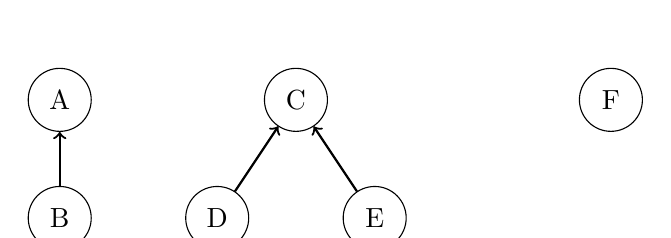
\begin{tikzpicture}[
        level distance=1.5cm,
        level 1/.style={sibling distance=2cm},
        every node/.style={circle, draw, minimum size=0.8cm}
    ]
    
    % First tree (A with child B)
    \node (A) at (0,0) {A}
        child {node (B) {B}};
    
    % Second tree (C with children D and E)
    \node (C) at (3,0) {C}
        child {node (D) {D}}
        child {node (E) {E}};
    
    % Third tree (just F)
    \node (F) at (7,0) {F};
    
    % Arrows from children to parent roots
    \draw[->, thick] (B) -- (A);
    \draw[->, thick] (D) -- (C);
    \draw[->, thick] (E) -- (C);
    
    \end{tikzpicture}
    \caption{A forest where there are three trees with representatives A, C and
    F.}
    \label{fig:forest}
\end{figure}

\begin{figure}[H]
    \centering  
    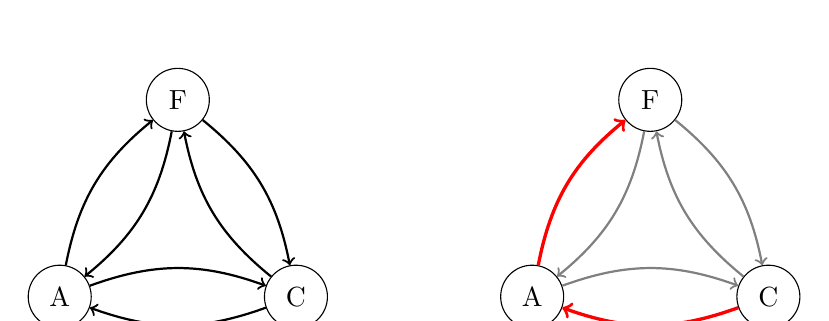
\begin{tikzpicture}[
        every node/.style={circle, draw, minimum size=0.8cm},
        every edge/.style={draw, ->, thick}
    ]
    
    % First graph
    \begin{scope}
        % Position the three nodes in a triangle
        \node (A) at (0,0) {A};
        \node (C) at (3,0) {C};
        \node (F) at (1.5,2.5) {F};
        
        % Create cycles with arrows
        \draw[->, thick] (A) to[bend left=20] (C);
        \draw[->, thick] (C) to[bend left=20] (A);
        
        \draw[->, thick] (C) to[bend left=20] (F);
        \draw[->, thick] (F) to[bend left=20] (C);
        
        \draw[->, thick] (F) to[bend left=20] (A);
        \draw[->, thick] (A) to[bend left=20] (F);
    \end{scope}
    
    % Second graph (shifted to the right with highlighted arrows)
    \begin{scope}[xshift=6cm]
        % Position the three nodes in a triangle
        \node (A2) at (0,0) {A};
        \node (C2) at (3,0) {C};
        \node (F2) at (1.5,2.5) {F};
        
        % Create cycles with arrows (normal)
        \draw[->, thick, gray] (A2) to[bend left=20] (C2);
        \draw[->, thick, red, very thick] (C2) to[bend left=20] (A2);  % Highlighted C -> A
        
        \draw[->, thick, gray] (C2) to[bend left=20] (F2);
        \draw[->, thick, gray] (F2) to[bend left=20] (C2);
        
        \draw[->, thick, gray] (F2) to[bend left=20] (A2);
        \draw[->, thick, red, very thick] (A2) to[bend left=20] (F2);  % Highlighted A -> F
    \end{scope}
    
    \end{tikzpicture}
    \caption{On the left a graph of roots from Figure \ref{fig:forest}. On the right a conflict-free set highlighted in red.}
    \label{fig:conflict-free-set}
\end{figure}

\begin{figure}[H]
    \centering  
    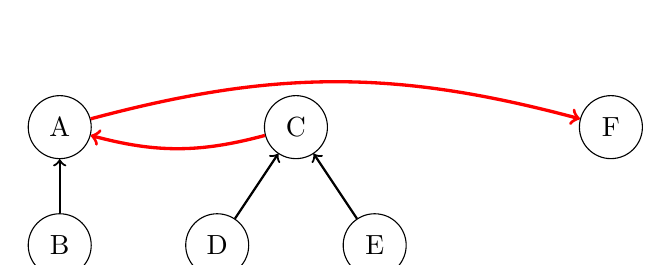
\begin{tikzpicture}[
        level distance=1.5cm,
        level 1/.style={sibling distance=2cm},
        every node/.style={circle, draw, minimum size=0.8cm}
    ]
    
    % First tree (A with child B)
    \node (A) at (0,0) {A}
        child {node (B) {B}};
    
    % Second tree (C with children D and E)
    \node (C) at (3,0) {C}
        child {node (D) {D}}
        child {node (E) {E}};
    
    % Third tree (just F)
    \node (F) at (7,0) {F};
    
    % Original arrows from children to parent roots
    \draw[->, thick] (B) -- (A);
    \draw[->, thick] (D) -- (C);
    \draw[->, thick] (E) -- (C);
    
    % New highlighted edges
    \draw[->, very thick, red] (A) to[bend left=15] (F);
    \draw[->, very thick, red] (C) to[bend left=15] (A);
    
    \end{tikzpicture}
    \caption{The forest from Figure \ref{fig:forest} after adding the
    conflict-free set from Figure \ref{fig:conflict-free-set}.}
    \label{fig:forest-after-conflict-free}
\end{figure}
\noindent The formal definition of a conflict-free set is as previous described
a set of root pairs that forms a forest.
\begin{definition}[Conflict-free Set]
  Let $F$ be a forest, $X \subseteq \{(\rho_F(v), \rho_F(u)) : (v, u) \in V
  \times V\}$ be a set of root pairs. Then $X$ is a conflict-free set in $F$
  if $(V, Y)$ is a forest.
\end{definition}
\noindent With this definition of a conflict-free set we now wish to show that
we can add all edges in a conflict-free set to a forest and still have a forest.
\begin{proposition}[Conflict-free Forest Union]\label{prop:conflict-free-forest-union}
  Let forest $F = (V, E)$ be a forest and let $X \subseteq V \times V$ be a
  conflict-free set in $F$ where $|X| = n$. Then defining the following forests:
  \begin{align*}
    F_0 &:= F \\
    F_{i} &:= (V, E_{i - 1} \cup \{(v_i, u_i)\}) \text{ for } (v_i, u_i) \in X \text{ and } 1 \leq i \leq n
  \end{align*}
  Then $F_n$ is a forest.
\end{proposition}

\begin{proof}
  Let forest $F = (V, E)$ be a forest, $X \subseteq V \times V$ be a
  conflict-free set in $F$. We will show that $F_n$ is a forest by induction
  on $i$.
  \begin{itemize}
    \item Base case: If $i = 0$ then $F_i = F_0 = F$ which is a forest.
    \item Induction hypothesis: Assume that $F_{i - 1}$ is a forest for all
    $1 \leq i < n$.  Let $(v_i, u_i) \in X$, we know that $v_i \neq v_j$ for
    all $(v_j, u_j) \in Y \backslash \{(v_i, u_i)\}$ since otherwise $(V,
    X)$ would not be a forest and $X$ would not be a conflict-free set in
    $F$. So $v_i$ will only have one parent in $F_i$ since it only appears
    once as a child in $(V, X)$. By definition all of the edges in $X$
    consists of roots in $F$, and since $(V, X)$ is a forest there are no
    cycles $y \centernot\leadsto y$ for all $y \in V$ in $F_i$. Hence $F_i$
    is a forest.
  \end{itemize}
  Thus by induction $F_n$ is a forest.
\end{proof}
\noindent We also need to show that Conflict-free Forest Union
\ref{prop:conflict-free-forest-union} satisfies Tree Union Property
\ref{def:tree-union-property}. This is done by showing that adding edges from
the conflict-free set to a forest in any order is equivalent to adding each edge
in the same order using Root Union \ref{prop:root-union}.
\begin{proposition}[Conflict-free Set Equivalence]\label{prop:conflict-free-set-equivalence}
  Let forest $F$ be a forest and let $X \subseteq V \times V$ be a
  conflict-free set in $F$ where $|X| = n$. Then defining the following forests:
  \begin{align*}
    F_0 &:= F \\
    F_{i} &:= (V, E_{i - 1} \cup \{(v_i, u_i)\}) \text{ for } (v_i, u_i) \in X \text{ and } 1 \leq i \leq n \\
    G_0 &:= F \\
    G_{j} &:= (V, E_{i - 1} \cup \{(\rho_{G_{j - 1}}(v_j), \rho_{G_{j - 1}}(u_j))\}) \text{ for } (v_j, u_j) \in X \text{ and } 1 \leq j \leq n
  \end{align*}
  Then $F_{n} \cong G_{n}$.
\end{proposition}
\begin{proof}
  Let $F$ be a forest, $X \subseteq V \times V$ be a conflict-free set in $F$.
  We will show that $F_n \cong G_n$. We know that for some $(v_i, u_i) \in X$
  then $v_i \neq y$ for all  $(y, w) \in X \backslash \{(v_i, u_i)\}$ since
  otherwise $(V, X)$ would not be a forest and $X$ would not be a conflict-free
  set in $F$. So all edge set unions will only give a root $v_i$ a new parent
  $u_i$ once. So $\rho_{F_n}(v_i) = \rho_{F_n}(u_i)$ and $\rho_{G_n}(u_i) =
  \rho_{G_n}(v_i)$ hence $v_i$ remains in the same tree in both $F_n$ and $G_n$.
  Since this holds for all $(v_i, u_i) \in X$ it follows that all elements in
  $V$ remains in the same tree in both $F_n$ and $G_n$. Hence $F_n \cong G_n$.
\end{proof}
\noindent From this equivalence it will be shown that Conflict-free Forest Union
\ref{prop:conflict-free-forest-union} satisfies Tree Union Property
\ref{def:tree-union-property}.
\begin{corollary}[Conflict-free Union Satisfies Tree Union
  Property]\label{cor:conflict-free-union-satisfies-tree-union-property} Let
  forest $F$ be a forest and let $X \subseteq V \times V$ be a conflict-free set
  in $F$ where $|X| = n$. Then defining the following forests:
  \begin{align*}
    F_0 &:= F \\
    F_{i} &:= (V, E_{i - 1} \cup \{(v_i, u_i)\}) \text{ for } (v_i, u_i) \in X \text{ and } 1 \leq i \leq n
  \end{align*}
  Then for all $(v_i, u_i) \in X$ it holds that $v_i \sim_{F_n} u_i$ and $F_n$
  satisfies the properties of a tree union.
\end{corollary}
\begin{proof}
  Let forest $F$ be a forest, $X \subseteq V \times V$ be a conflict-free set
  in $F$. By proposition \ref{prop:conflict-free-set-equivalence} it holds
  that $F_n \cong G_n$ where $G_n$ is defined as in proposition
  \ref{prop:conflict-free-set-equivalence}. By proposition \ref{prop:root-union}
  it holds that for all $(v_i, u_i) \in X$ then $v_i \sim_{G_n} u_i$ and $G_n$
  satisfies the properties of a tree union. Since $F_n \cong G_n$ it follows
  that for all $(v_i, u_i) \in X$ then $v_i \sim_{F_n} u_i$ and $F_n$ satisfies
  the properties of a tree union.
\end{proof}

\noindent Now that we have established the properties of conflict-free sets we
can now define a method to find a conflict-free set from a set of root pairs.
The method chosen to find a conflict-free set is to consider an directed acyclic
graph. Such a graph fulfills one property of a forest, namely that there are no
cycles. This is ensured by ordering the edges in the graph such that for all
edges $(v, u)$ it holds that $v < u$ for some strict total order $(V, <)$. We
may do this since the equivalence classes in a forest can be represented by any
representative in the tree. Hence we can alwauys pick a total order on the
vertices in the forest.
\begin{proposition}[Ordered Edges Implies Acyclicity]\label{prop:ordered-edges-implies-acyclicity}
  Let $G = (V, E)$ be a directed graph where for all $(v, u) \in E$ it holds
  that $v < u$ for some strict total order $(V, <)$. Then $G$ has no cycles.
\end{proposition}

\begin{proof}
  Let $G = (V, E)$ be a directed graph where for all $(u, v) \in E$ it holds
  that $u < v$ for some total order $(V, <)$. Let edges $e_1, e_2, \ldots, e_m
  \in E$ where $m \geq 1$ and $e_i = (v_{i-1}, v_i)$ for $1 \leq i \leq m$ be
  some path in $G$. Since the edges are ordered it follows that:
  \begin{align*}
    v_0 < v_1 < v_2 < \cdots < v_{m - 1} < v_m
  \end{align*}
  Hence by transitivity of the total order it follows that $v_0 < v_m$. So
  $v_0 \neq v_m$ hence there are no cycles in $G$.
\end{proof}
\noindent The nice property of using a directed acyclic graph is we can now pick
out any edges from the graph such that no two edges have the same child. This
will ensure that the picked out edges forms a forest.

\subsection{Parallel Union-Find}
The conflict-free sets makes it is possible to define how unification in the
union-find strucutre works. If we consider that we have some forest $F = (V, E)$
and then are given a set of vertex pairs $A \subseteq V \times V$ we wish to
unify these pairs such that they are equivalent in some forest $F$. We can turn
$A$ into an directed acyclic graph $(V, Z)$ where $Z$ only consists of root
pairs from $F$. We want to pick out a subset of $Z$ such that we unify as many
of the vertex pairs of $Z$ in $F$ as possible leading to a good time complexity
of the algorithm. All of these pairs can not be unified immediately so an
algorithm will be first derived which picks out a subset of the directed acyclic
graph $(V, Z)$ and then unifies them in $F$. To determine what a large set is,
we first need to define a notion of an edge cover that can be serve as a measure
of how many vertex pairs in $Z$ can be unified:
\begin{definition}[Edge Cover]
    Let $V$ be a set and $E \subseteq V \times V$ such that $\pi_1(E) \cup
    \pi_2(E) = V$ then $E$ is an edge cover of $V$.
\end{definition}
\noindent Using this definition we know that $V' = \pi_1(Z) \cup \pi_2(E)$ is an
edge cover of the subgraph $(V', Z)$ of $(V, Z)$. Why this is relevant is that
vertices in $V\backslash V'$ will not be unified so they are not relevant during
unification. Futhermore, the bound that will be established is for every
iteration then atleast $\frac{|V'|}{2}$ vertices must be unified. The intuition
behind this is that every time a vertex is given a parent then it can not be
given a parent later so it has been dealt with. We can show that when we have
such an edge cover then the following inequality holds:
\begin{proposition}[Edge Cover Inequality]\label{prop:set-2-tuple-inequality}
    Let $V$ be a set and $E \subseteq V \times V$ be a edge cover of V then: 
    \begin{align*}
        |\pi_1(E)| < \frac{|V|}{2} \implies |\pi_2(E)| > \frac{|V|}{2} 
    \end{align*}
\end{proposition}
\begin{proof}
    Let $V$ be a set and $E \subseteq V \times V$ be a edge cover of V, and
    $|\pi_1(E)| < \frac{|V|}{2}$. Let $A = \pi_1(E) = \{v : (v, u) \in E\}$, $B
    = \pi_2(E) = \{u : (v, u) \in E\}$ and $C = B \backslash A$. By definition of $C$ we
    have $A \cap C = \emptyset$ so $|A| + |C| = |V|$ and since $|B| \geq |C|$ we
    can conclude that:
    \begin{align*}
        |B| \geq |C| = |V| - |A| > |V| - \frac{|V|}{2} = \frac{|V|}{2}
    \end{align*}
    Hence $|\pi_1(E)| > \frac{|V|}{2}$.
\end{proof}
\noindent This inequality tells us that if $Z$ does not resolve enough vertices,
then if we invert the edges in $Z$ then it would be possible to resolve enough
vertices. It just remains to show that inverting these edges direction will
still give an directed acyclic graph.  
\begin{proposition}[Inverted Acyclic Graph is Acyclic]\label{prop:inverted-acyclic-graph}
  Let $G = (V, E)$ be a directed acyclic graph. Then the inverted graph $G' =
  (V, E')$ where $E' = \{(u, v) : (v, u) \in E\}$ is also acyclic.
\end{proposition}
\begin{proof}
  Let $G = (V, E)$ be a directed acyclic graph and $G' = (V, E')$ where $E' =
  \{(u, v) : (v, u) \in E\}$ is the inverted graph. Let edges $e_1, e_2,
  \ldots, e_m \in E'$ where $m \geq 1$ and $e_i = (v_{i-1}, v_i)$ for $1 \leq
  i \leq m$ be some path in $G'$. By definition of $E'$ it follows that there
  exists edges $e'_1, e'_2, \ldots, e'_m \in E$ where $e'_i = (v_i, v_{i-1})$
  for $1 \leq i \leq m$. If there was a cycle in $G'$ then it would hold that
  $v_0 = v_m$. But since $G$ is acyclic it follows that $v_0 \neq v_m$. Hence
  there are no cycles in $G'$.  
\end{proof}
\noindent The algorithm which tries to unifies atleast $\frac{|V'|}{2}$ can now
be defined. It starts by determining if the directed acyclic subgraph $(V', Z)$
should be inverted as to give $\frac{|V'|}{2}$ vertices a parent. Afterwards 
just pick out as many pairs with a unique child.
\begin{algorithm}[Maximal Union]\label{alg:maximal-union} Let forest $F = (V,
  E)$ be a forest and let $Z \subseteq \{(\rho_F(v), \rho_F(u)) : (v, u) \in V
  \times V\}$ be a set of root pairs $F$ and $(V, Z)$ is an acyclic directed
  graph. The maximal union algorithm is defined as:
  \begin{align*}
    & \id{MaximalUnion}(F, Z) \\ 
    1. & \qquad (V, E) \leftarrow F \\
    2. & \qquad V' \leftarrow \pi_1(Z) \cup \pi_2(Z) \\
    3. & \qquad Z \leftarrow \begin{cases}
      \{(u, v) : (v, u) \in Z\} & \pi_1(Z) < \frac{|V'|}{2} \\
      Z & \pi_1(Z) \geq \frac{|V'|}{2}
    \end{cases} \\
    4. & \qquad X \leftarrow Y \subseteq Z \text{ where } |Y| = |\pi_1(Z)| \text{ and } \pi_1(Y) = \pi_1(Z) \\
    5. & \qquad G \leftarrow (V, X) \\
    6. & \qquad E \leftarrow E \cup \{(v, \rho_G(u)) : (v, u) \in X\} \\
    7. & \qquad \kw{return} \: ((V, E), Z \backslash X)
  \end{align*}
\end{algorithm}
\noindent By definition we can clearly see atleast $\frac{|V'|}{2}$ vertices are
given a parent as we wanted. It will now be shown that the added edges is a
conflict-free set so a forest is still the result.
\begin{proposition}[Maximal Union
  Correctness]\label{prop:maximal-union-correctness} Let forest $F = (V, E)$ be
  a forest and let $Z \subseteq \{(\rho_F(v), \rho_F(u)) : (v, u) \in V \times
  V\}$ be a set of root pairs $F$ and $(V, Z)$ is an acyclic directed graph.
  Then the maximal union algorithm results in a forest $F' = (V, E')$ which
  satifies the Tree Union Property \ref{def:tree-union-property} for the
  conflict-free set $X \subseteq Z$ in $F$.
\end{proposition}
\begin{proof}
  Let forest $F = (V, E)$ be a forest and let $Z \subseteq \{(\rho_F(v),
  \rho_F(u)) : (v, u) \in V \times V\}$ be a set of root pairs $F$ and $(V, Z)$
  is an acyclic directed graph. From proposition
  \ref{prop:inverted-acyclic-graph} we know that $(V, Z)$ remains an acyclic
  graph throughout the algorithm. Since $X$ is defined such that $\pi_1(X) =
  \pi_1(Z)$ and $|X| = |\pi_1(Z)|$ it follows that $X$ is a conflict-free set in
  $F$ since no vertex $v$ appears more than once as a child in $X$ i.e. $G = (V,
  X)$ is a forest. We can also conclude that $(V, \{(v, \rho_G(u)) : (v, u) \in
  X\}) \cong (V, X)$ since every child directly points to its root. So adding
  the edges in $\{(v, \rho_G(u)) : (v, u) \in X\}$ to $E$ it follows by
  corollary \ref{cor:conflict-free-union-satisfies-tree-union-property} that the
  algorithm fulfills the Tree Union Property \ref{def:tree-union-property} and
  $F' = (V, E')$ where $E' = E \cup \{(v, \rho_G(u)) : (v, u) \in X\}$.
\end{proof}
\noindent Before the time complexity of maximal union can be shown the time
complexity of path comopression has to be discussed. A problem that occur in the
analysis is the computation of $\{(v, \rho_G(u)) : (v, u) \in X\}$. Since the
forest $(V, X)$ that may be constructed could be just a tree which is one long
chain so $\rho_G(u)$ does $O(|X|)$ work to find its parent. This problem can be
solved using pointer jumping, specifically Wyllie's List Ranking algorithm
\cite[59]{wyllie1979complexity} can be used directly on a forests to do $O(n
\log n)$ work with $O(\log n)$ span on a forest of $n$ vertices. This is not
work-efficient, you would want to do $O(n)$ work. There are list ranking
algorithms \cite{Anderson1991} which are work-efficient with $O(\log^2 n)$
span\footnote{They assume scan has $O(1)$ span which is not reasonable
anymore.}. List ranking can be used to construct an euler tour of an edge
list\footnote{\url{https://www.cs.cmu.edu/~scandal/nesl/algorithms.html\#trees}},
this euler tour represents a V-Tree \cite[84-91]{Blelloch1990} and this method
will work on a forests. It is not clear if this method can be avoided and
instead just directly applying the list ranking on the forest as to avoid alot
of work. This can atleast be done with Wyllies List ranking. It also seems that
using a connected components algorithm by Shiloach and Vishkin
\cite{SHILOACH198257} could be used which will give you a representative, it
claims to be work-efficient with $O(\log n)$ span but uses a computational model
with concurrent write. This may or may not be a problem to express this in a
parallel functional array language but there are implementations in NESL \cite{spaa-concomp}.

\begin{proposition}[Maximal Union Time
  Complexity]\label{prop:maximal-union-time-complexity} Let forest $F = (V, E)$
  be a forest and let $Z \subseteq \{(\rho_F(v), \rho_F(u)) : (v, u) \in V
  \times V\}$ be a set of root pairs in $F$ and $(V, Z)$ is an acyclic directed
  graph. Then the maximal union algorithm runs in $O(|Z|)$ work and $O(\log^2
  |Z|)$ depth.
\end{proposition}

\begin{proof}
  For step 1. it takes $O(1)$ work and $O(1)$ if we assume that $E$ is only used
  once in this function. Step 2-3. finds unique elements and can be computed
  with a parallel integer sort and a filter, assuming the encoding of vertices
  uses a fixed number of $k$-bits then this part is $O(|Z|)$ work and $O(\log
  |Z|)$ span. Step 4. can be implemented by a parallel integer sort on the first
  element of each pair in $Z$ followed by a parallel filter that selects the
  first occurrence of each unique first element, this takes $O(|Z|)$ work and
  $O(\log |Z|)$ depth. Step 6. takes $O(|X|)$ work and $O((\log |X|)^2)$ depth
  to do path compression and add these edges to $E$. Step 7. takes $O(|Z|)$ work
  and $O(\log |Z|)$ depth to compute the set difference $Z \backslash X$ by a
  filter. Hence the total work is $O(|Z|)$ and the total depth is $O(\log |Z|)$.
  Hence the maximal conflict-free set algorithm runs in $O(|Z|)$ work and
  $O((\log |Z|)^2)$ depth.
\end{proof}
\noindent Now the time complexity is known we can finally give the algorithm for
parallel union which performs bulk unification making a set of $A$ pair vertices
become equivalent in the final forest. The way the algorithm works is by
constructing a directed acyclic graph of roots from $A$ which will be called
$Z$. Then have a loop with the invariant that $(V, Z)$ is an directed
acyclic graph. Then in the loop body simply perform maximal union and turn the
remaining uninserted edge of $Z$ into an directed acyclic graph. Continue till
$Z$ is empty and then $F$ is the final forest where all pairs of $A$ has been
unified.

\begin{algorithm}[Parallel Tree Union]\label{alg:parallel-tree-union} Let forest
  $F = (V, E)$ be a tree and let $A \subseteq V \times V$ be a set of pairs of
  elements in $V$ that will be unified in parallel. The parallel tree union
  algorithm is defined as:
  \begin{align*}
    & \id{ParallelTreeUnion}(F, A) \\
    1. & \qquad Z_p \leftarrow \{(\rho_F(v), \rho_F(u)) : (v, u) \in A \land \rho_F(v) \neq \rho_F(u)\} \\
    2. & \qquad Z \leftarrow \{(\min \{v, u\}, \max \{v, u\}) : (v, u) \in Z_p\} \\
    3. & \qquad \kw{while }~|Z| > 0~\kw{do} \\
    4. & \quad \qquad (F, Z_q) \leftarrow \id{MaximalUnion}(F, Z) \\
    5. & \qquad \quad Z_r \leftarrow \{(\rho_{F}(v), \rho_{F}(u)) : (v, u) \in Z_q \land \rho_{F}(v) \neq \rho_{F}(u)\} \\
    6. & \qquad \quad Z \leftarrow \{(\min \{v, u\}, \max \{v, u\}) : (v, u) \in Z_r\} \\
    7. & \qquad \kw{return} \: F
  \end{align*}
\end{algorithm}
\noindent First of all we have to establish that the actual algorithm produces
the correct output, as in it fullfills the Tree Union property \ref{def:tree-union-property}.

\begin{proposition}[Parallel Tree Union Correctness]\label{prop:parallel-tree-union-correctness}
  Let forest $F = (V, E)$ be a tree and let $A \subseteq V \times V$ be a set of
  pairs of elements in $V$ that will be unified in parallel. Then the parallel
  tree union algorithm results in a forest $F' = (V, E')$ which satifies the
  Tree Union Property \ref{def:tree-union-property} for $A$.
\end{proposition}
\begin{proof}
  To show that the algorithm returns a forest $F' = (V, E')$ where for all $(v,
  u) \in A$ it holds that $v \sim_{F'} u$ it will be shown that the steps in the
  algorithm does not remove unification problems $(v, u) \in A$ which do not
  hold at some step in the final forest $F$.

  First in step. 1-2 creates a directed acyclic graph $(V, Z)$ which represents
  the same unification problems as in $A$. Since if $\rho_F(v) = \rho_F(u)$
  where $(v, u) \in A$ then $v \sim_{F} u$ so $u$ and $v$ have already been
  unified. Secondly reordering the components of $(v, u)$ does not change the
  since adding an edge $(u, v)$ or $(v, u)$ to a forest commutes since $v
  \sim_{F} u$ commutes.
  
  The loop in Step. 3-6 has the following invariant that $Z$ is an directed
  acyclic graph. It will be shown that this invariant is fulfilled and that
  implies $F$ fulfills $v \sim_{F} u$ for all $(v, u) \in A$ in the final $F$.
  In the start of the loop the acylic directed graph invariant holds. Then in
  step 4. using Maximal Union \ref{alg:maximal-union} achieves a forest with a
  proper subset of $Z$ being unified and $Z_q$ is the remaining pairs that have
  not been unified. In step 5-6. the directed acyclic graph $Z$ is constructed
  (by the same arguments as in step 1-2.) from $Z_q$ fulfilling the loop
  invariants.

  Since the loop continuesly unifies using Maximal Union on the remaining
  unification problems then the algorithm does fulfill the Tree Union property
  \ref{def:tree-union-property}.
\end{proof}
\noindent Before giving the general analysis of union find a specicial case of
when the initial forest is $F = (V, \emptyset)$. Since this is a likely case
that can happen for certain algorithms.
\begin{proposition}[Empty Parallel Tree Union Time
  Complexity]\label{prop:empty-time-complexity} Let forest $F = (V, \emptyset)$
  be a tree, and let $A \subseteq V \times V$ be a set of pairs of elements in
  $V$ that will be unified in parallel. Then the parallel tree union algorithm
  does $O(|A|)$ work and has $O(\log^3 |A|)$ span.
\end{proposition}

\begin{proof}
  Let forest $F = (V, \emptyset)$ be a tree, step 1-2. a filter and an ordering
  is applied which can be computed in $O(|A|)$ work and $O(\log |A|)$ span. This
  is the time complexity since $\rho_F(v)$ and $\rho_F(u)$ is $O(1)$ work and
  span so the maximum traversals to root is constant.
  
  The body of the loop at step 4-6 does at first $O(|Z|)$ work and $O(\log^2
  |Z|)$ span where $|Z|$. The factor is dominated by Maximal Unions time
  complexity \ref{prop:maximal-union-time-complexity} due to 5-6 being a filter
  and the map. Since the search of the representative element is $O(1)$ because
  the path compression in maximal union will make the distance to the
  representative be at most $1$.

  The amount of vertices removed from $V' = \pi_1(Z) \cup \pi_2(Z)$ in the next
  iteration is lowerbounded by $\frac{|V'|}{2}$ due to maximal union
  \ref{alg:maximal-union}. These remaining vertices are used to construct a
  directed acyclic graph $(V', Z')$ where $Z' \subseteq V' \times V'$. We can
  establish the following bound of $Z'$ using the fact that $\binom{n}{2}$ is
  the upperbound for a directed acyclic graphs size of $n$ vertices. 
  \begin{align*}
    |Z'| \leq \binom{\frac{|V'|}{2}}{2} = \frac{\left(\frac{|V'|}{2}\right)^2 - \frac{|V'|}{2}}{2} = \frac{\frac{1}{2}|V'|^2 - |V'|}{4} 
  \end{align*}
  Now if we consider the half amount of edges that $(V', Z')$ can maximally have
  $\frac{\binom{|V'|}{2}}{2}$ the following inequality arises. 
  \begin{align*}
    |Z'| \leq \frac{\frac{1}{2}|V'|^2 - |V'|}{4} \leq \frac{|V'|^2 - |V'|}{4} = \frac{\binom{|V'|}{2}}{2}
  \end{align*}
  Meaning that by halving the amount of $V'$ every iteration is bounded by
  halving the amount of $Z'$ worked on each iteration of the loop. Since
  $|Z'|$ is upperbounded by $|A|$ we get the total work done by the loop is:
  \begin{align*}
    \sum^{\lfloor \log |A| \rfloor}_{k = 0} \frac{|A|}{2^k} = 
    |A| \sum^{\lfloor \log |A| \rfloor}_{k = 0} \frac{1}{2^k} < 
    |A| \sum^{\infty}_{k = 0} \frac{1}{2^k} = 2|A|
  \end{align*}
  Meaning the work of the function is $O(|A|)$. The span is $O(\log^3 |A|)$
  since the worst span is by maximal union $O(\log^2 |A|)$ which is done $O(\log
  |A|)$ times.
\end{proof}
\noindent The time complexity is good for certain cases, but in the general case
for any forests, the time complexity becomes way worse.
\begin{proposition}[Parallel Tree Union Time
  Complexity]\label{prop:parallel-tree-union-time-complexity} Let forest $F =
  (V, E)$ be a tree, and let $A \subseteq V \times V$ be a set of pairs of
  elements in $V$ that will be unified in parallel. Given $k$ applications of
  Parallel Tree Union \ref{alg:parallel-tree-union} before then Parallel Tree
  Union does $O(|A| k \log |V|)$ work and has $O(k \log |V| + \log^3 |A|)$ span.
\end{proposition}
\begin{proof}
  The analysis is the same as in the empty case \ref{prop:empty-time-complexity}
  beside in step 1. Considering a sequence of unification problems that have
  been unified $A_1, A_2, \ldots, A_k$. In the worst case then $|A_i|$ will
  extened upon a trees height by $\lfloor \log |\pi(A_i) \cup \pi_2(A_i)|
  \rfloor$ since the alogrithm half the number of vertices every iteration of
  $|A|$ in the worst case. since $|\pi(A_i) \cup \pi_2(A_i)| \leq |V|$ the
  following bound can be derived on a sequence of unification problems.
  \begin{align*}
    \sum_{i = 1}^k \lfloor \log |\pi(A_i) \cup \pi_2(A_i)| \rfloor \leq \sum_{i = 1}^k  \lfloor \log |V| \rfloor = k \lfloor \log |V| \rfloor
  \end{align*}
  Therefore we can conclude the amount the work is $O(|A| k \log |V|)$ and the
  span is $O(k \log |V| + \log^3 |A|)$
\end{proof}
\noindent Now we can go on to consider the asymptotics of performing a find. 
\begin{proposition}[Parallel Tree Find Time Complexity]
  Let forest $F = (V, E)$ be a tree and let $v \in V$ be a element in $V$ which
  representative will be found. Given $k$ applications of Parallel Tree Union
  \ref{alg:parallel-tree-union} then find does $O(k \log |V|)$ work and has $O(k
  \log |V|)$ span.
\end{proposition}
\begin{proof}
  Using the proof of Parallel Tree Find Time Complexity
  \ref{prop:parallel-tree-union-time-complexity} where it was shown that the
  tree height is upperbounded by $k \lfloor \log |V| \rfloor$ after $k$
  applications of parallel tree union. Hence finding a single elements
  representative will have $O(k \log |V|)$ work and span.
\end{proof}

\subsection{Union by Size and Rank}
The next problem is to extend the data-parallel union-find structure such that
it would allow the usage of the union by size or rank heurestic. To do this
graph $(V, E)$ with weighted vertices is introduced where the weight is given by
a function $f : V \to \mathbb{N}$. We may update a functions range by $f' = f
\oplus S$ where $S \subseteq V \times \mathbb{N}$ where the pair $(v, n) \in S$
with the maximum $n$ becomes the result of $v$ i.e. $f'(v) = n$. Now using this
we wish to show that it is possible to establish an total ordering on $f(v)$
where if $f(v) = f(u)$ then it default to ordering by the values given to $f$.

\begin{proposition}[Weighted Total Ordering]
  Let $V$ be a total ordering set $(V, \lesssim)$ and $f : V \to \mathbb{N}$ then
  $(v, \preceq_f)$ is a total ordering where
  \begin{align*}
    v \preceq_f u \begin{cases}
      f(v) < f(u) & f(v) < f(u) \\
      v \lesssim u & f(v) = f(u)
    \end{cases}
  \end{align*}
\end{proposition}
\begin{proof}
  To show it is a total ordering it must be shown that the relation is
  reflexive, transitive, antisymmetric, and total.
  \begin{enumerate}
    \item If $v \preceq_f v$ holds  then $f(v) = f(v)$ holds and so does $v \lesssim v$.
    \item If $v \preceq_f u$ and $u \preceq_f w$ holds then:
    \begin{itemize}
      \item If $f(v) < f(u) < f(w)$ holds then $v \preceq_f w$.
      \item If $f(v) = f(u) = f(w)$ holds then $v \preceq_f w$.
      \item If $f(v) < f(u) = f(w)$ holds then $v \preceq_f w$.
      \item If $f(v) = f(u) < f(w)$ holds then $v \preceq_f w$.
    \end{itemize}
    \item If $v \preceq_f u$ and $u \preceq_f v$ holds then $f(v) < f(u)$ and $f(v)
    > f(u)$ can not hold so $f(v) = f(u)$. So $v \lesssim u$ and $u \lesssim v$
    both holds and since $(V, \lesssim)$ is a total ordering then $v = u$.
    \item Since $(\mathbb{N}, \leq)$ then either $f(v) < f(u)$, $f(u) < f(v)$,
    or $f(v) = f(u)$ holds. First case yields $v \preceq_f u$, second case yields
    $u \preceq_f v$. Last case yields either $v \lesssim u$ or $v \lesssim u$,
    since $(V, \lesssim)$ is total then either $v \preceq_f u$ or $v \preceq_f u$
    holds making the relation total.
  \end{enumerate}
\end{proof}
\noindent The idea now is to have $f$ be a function which reflects the rank/size
of a vertex and then create the directed acyclic graph from a set of root pairs.
Then it is possible to pick conflict-free set and insert this into the forest
which will respect the weights limiting the height of the trees. For this
algorithm it has two different was of being instantiated, either with the by
rank or by size heurestic. This modifies maximal union and parallel union quite
a bit.
\begin{algorithm}[Weighted Maximal Union]\label{alg:weighted-maximal-union} Let
  forest $F = (V, E)$ be a forest, $f: V \to \mathbb{N}$ and let $Z \subseteq
  \{(\rho_F(v), \rho_F(u)) : (v, u) \in V \times V\}$ be a set of root pairs $F$
  and $(V, Z)$ where $v \preceq_f u$ and $v \neq u$ for all $(v, u) \in Z$. The
  weighted maximal union algorithm is defined as:
  \begin{align*}
    & \id{WeightedMaximalUnion}(F, Z, f) \\ 
    1. & \qquad (V, E) \leftarrow F \\
    2. & \qquad A \leftarrow \{(v, u) : (v, u) \in Z \land f(v) = f(u)\} \\
    3. & \qquad B \leftarrow \{(v, u) : (v, u) \in Z \land f(v) \neq f(u)\} \\
    4. & \qquad V' \leftarrow \pi_1(A) \cup \pi_2(A) \\
    5. & \qquad A \leftarrow \begin{cases}
      \{(u, v) : (v, u) \in A\} & \pi_1(A) < \frac{|V'|}{2} \\
      A & \pi_1(A) \geq \frac{|V'|}{2}
    \end{cases} \\
    6. & \qquad Z \leftarrow A \cup B \\
    7. & \qquad X \leftarrow Y \subseteq Z \text{ where } |Y| = |\pi_1(Z)| \text{ and } \pi_1(Y) = \pi_1(Z) \\
    8. & \qquad G \leftarrow (V, X) \\
    9. & \qquad X \leftarrow \{(v, \rho_G(u)) : (v, u) \in X\} \\
    10. & \qquad E \leftarrow E \cup X \\
    11. & \qquad f \leftarrow f \oplus \{(v, f(u) + 1) : (v, u) \in X \land f(v) = f(u)\}  \quad (\text{By Rank}) \\
    11. & \qquad f \leftarrow f \oplus \left\{\left(v, \sum_{(v, u) \in X} f(u)\right) : v \in V\right\} \quad (\text{By Size}) \\
    12. & \qquad \kw{return} \: ((V, E), Z \backslash X, f)
  \end{align*}
\end{algorithm}
\begin{proposition}[Weighted Maximal Union
  Correctness]\label{prop:weighted-maximal-union-correctness} Let forest $F =
  (V, E)$ be a forest, $f: V \to \mathbb{N}$ and let $Z \subseteq \{(\rho_F(v),
  \rho_F(u)) : (v, u) \in V \times V\}$ be a set of root pairs $F$ and $(V, Z)$
  where $v \preceq_f u$ and $v \neq u$ for all $(v, u) \in Z$. Then the weighted
  maximal union algorithm results in a forest $F' = (V, E')$ which satifies the
  Tree Union Property \ref{def:tree-union-property} for the conflict-free set $X
  \subseteq Z$ in $F$.
\end{proposition}
\begin{proof}
  Let forest $F = (V, E)$ be a forest and let $Z \subseteq \{(\rho_F(v),
  \rho_F(u)) : (v, u) \in V \times V\}$ be a set of root pairs $F$ and $(V, Z)$
  be a set of root pairs $F$ and $(V, Z)$ where $v \preceq_f u$  and $v \neq u$
  for all $(v, u) \in Z$. By Proposition
  \ref{prop:ordered-edges-implies-acyclicity} we have that $(V, Z)$ is acyclic,
  and by partitioning $Z$ in to $A$ and $B$ and swapping edges in $A$ changes
  the relation from $(V, \lesssim)$ to $(V,\gtrsim)$ in $(V, \preceq_f)$ hence
  it is still a total ordering so $(V, A \cup B)$ is still acyclic. The
  algorithm will always remove at least one vertex from $\pi_1(Z) \cup \pi_2(Z)$
  since there must be atleast one unique vertex on the left hand side of any
  $(v, u) \in Z$. Therefore, the remaining of the algorithm does the same as in
  Maximal Union \ref{alg:maximal-union} hence the algorithm results in a forest
  $F' = (V, E')$ which satifies the Tree Union Property
  \ref{def:tree-union-property} for the conflict-free set $X \subseteq Z$ in $F$
  by Proposition \ref{prop:maximal-union-correctness}. The only way they differ
  is changing the function $f$ which is not of importance to the correctness.
\end{proof}
\noindent Now we find the time complexity of Weighted Maximal Union.
\begin{proposition}[Weighted Maximal Union Time
  Complexity]\label{prop:weighted-maximal-union-time-complexity} Let forest $F =
  (V, E)$ be a forest, $f : V \to \mathbb{N}$ be a function, and $Z \subseteq
  \{(\rho_F(v), \rho_F(u)) : (v, u) \in V \times V\}$ be a set of root pairs in
  $F$ and $(V, Z)$ is an acyclic directed graph. Then the maximal union
  algorithm runs in $O(|Z|)$ work and $O(\log^2 |Z|)$ depth.
\end{proposition}

\begin{proof}
  The arguments are almost the same as in Proposition
  \ref{prop:maximal-union-time-complexity}. The step 2-3 is just a partition and
  either of step 11. can be done using integer sorts and segmented reduce.
\end{proof}

\noindent Now we have to consider its corresponding parallel tree union
algorithm.
\begin{algorithm}[Weighted Parallel Tree
  Union]\label{alg:weighted-parallel-tree-union} Let forest $F = (V, E)$ be a
  tree, $f : V \to \mathbb{N}$ and let $A \subseteq V \times V$ be a set of
  pairs of elements in $V$ that will be unified in parallel. The weighted
  parallel tree union algorithm is defined as:
  \begin{align*}
    & \id{WeightedParallelTreeUnion}(F, A, f) \\
    1. & \qquad Z_p \leftarrow \{(\rho_F(v), \rho_F(u)) : (v, u) \in A \land \rho_F(v) \neq \rho_F(u)\} \\
    2. & \qquad Z \leftarrow \{(v, u) : (v, u) \in Z_p \land v \preceq_f u\} \cup \{(u, v) : (v, u) \in Z_p \land u \preceq_f v\} \\
    3. & \qquad \kw{while }~|Z| > 0~\kw{do} \\
    4. & \quad \qquad (F, Z_q, f) \leftarrow \id{WeightedMaximalUnion}(F, Z, f) \\
    5. & \qquad \quad Z_r \leftarrow \{(\rho_{F}(v), \rho_{F}(u)) : (v, u) \in Z_q \land \rho_{F}(v) \neq \rho_{F}(u)\} \\
    6. & \qquad \quad Z \leftarrow  \{(v, u) : (v, u) \in Z_r \land v \preceq_f u\} \cup \{(u, v) : (v, u) \in Z_r \land u \preceq_f v\}\\
    7. & \qquad \kw{return} \: F
  \end{align*}
\end{algorithm}
\noindent The correctness of weighted parallel tree union should be quite
evident but the proposition will be stated for completeness.
\begin{proposition}[Weighted Parallel Tree Union Correctness]\label{prop:weighted-parallel-tree-union-correctness}
  Let forest $F = (V, E)$ be a tree, $f : V \to \mathbb{N}$ and let $A \subseteq
  V \times V$ be a set of pairs of elements in $V$ that will be unified in
  parallel.  Then the weighted parallel tree union algorithm results in a forest
  $F' = (V, E')$ which satifies the Tree Union Property
  \ref{def:tree-union-property} for $A$.
\end{proposition}
\begin{proof}
  The proof follows mutatis mutandis from that of Proposition 
  \ref{prop:parallel-tree-union-correctness}.
\end{proof}
\noindent Now the time complexity of Weighted Parallel Tree Union will be
considered in regards to union by rank. Here we initially have $f(v) = 0$ for
all $v \in V$ and we now realize the following from definition of Weighted
Maximal Union by Rank that the weight of a representative $u$ only increase in
weight if $f(v) = f(u)$ for $(v, u)$ from a set of root pairs. 
\begin{remark}
  From the definition of the Weighted Maximal Union
  \ref{alg:weighted-maximal-union} the following follows. Let $F = (V, E)$, $f :
  V \to \mathbb{N}$, $(v, u) \in Z \subseteq \{(\rho_F(v), \rho_F(u)) : (v, u)
  \in V \times V\}$, $G = (V, Z)$ such that $\rho_{F'}(u) = \rho_{F'}(v) = u$
  where $F' = (V', E')$ is the forest as a result of the algorithm then
  the following holds.
  \begin{itemize}
    \item If $f(v) < f(u)$ for all $(v, u) \in Z$ then $(v, u) \in E'$ becomes
    the new forest and $f'$ is the new weight function where $f'(u) = f(u)$
    \item If $f(v) = f(u)$ for some $(v, u) \in Z$ then $(v, u) \in E'$ becomes
    the new forest and and $f'$ is the new weight function where $f'(u) = f(u) +
    1$.
  \end{itemize}
\end{remark}
\noindent Now to show that the time complexity is work-efficient first a bound
on the rank of every element is needed.
\begin{proposition}[Rank Bound]\label{prop:rank-bound} Let $F = (V, E)$, $f : V
  \to \mathbb{N}$, and $v \in V$, then the follow bound holds for all elements
  $v$ when used for union by rank.
  \begin{align*}
    f(v) \leq \lfloor \log |V| \rfloor
  \end{align*}
\end{proposition}
\begin{proof}
  It can be shown that the tree is bounded by $\lfloor \log k \rfloor$ given $k
  = |V|$ vertices using induction. The base case holds since given $1$ vertex
  $v$ then $f(v) = 0 \leq \lfloor \log k \rfloor$. Assume now the claim holds
  for $k$ vertices it will now be shown it holds for $k + 1$ vertices. So by the
  induction hypothesis $f(v), f(u) \leq \lfloor \log k \rfloor$ if $f(u) < f(v)$
  then for the new weight function $f'$ it must hold that $f'(v) = f(v) \leq
  \lfloor \log k \rfloor \leq \lfloor \log (k + 1) \rfloor$. If $f(v) = f(u) =
  h$ then $f'(v) = f(v) + 1$. By the induction hypothesis for $v, u \in V$ it
  holds that $f(v), f(u) \leq \lfloor \log k \rfloor$ so the height is bounded
  by $h$ meaning the subtrees $v$ and $u$ has at most $2^h$ vertices. Therefore,
  when unifying $v$ and $u$ with $v$ as the parent the final tree contains at
  least $2^h + 2^h = 2^{h + 1}$ vertices. Since the final tree has at most $k +
  1$ vertices it follows that $2^{h + 1} \leq k + 1$ and therefore $h + 1 = f(v)
  + 1 = f'(v) \leq \lfloor \log (k + 1) \rfloor$.
\end{proof}
\noindent Using the bound on ranks it is possible to derive the the time
complexity of the Weighted Parallel Tree Union algorithm when using the rank
heurestic.

\begin{proposition}[Weighted Parallel Tree Union (By Rank) Time
  Complexity]\label{prop:weighted-parallel-tree-union-time-complexity} Let
  forest $F = (V, E)$ be a tree, and let $A \subseteq V \times V$ be a set of
  pairs of elements in $V$ that will be unified in parallel. Then Weighted
  Parallel Tree Union does $O(|A| \log |V|)$ work and has $O((\log |V|)(\log^2
  |A|))$ span.
\end{proposition}
\begin{proof}
  In step 1. $O(|A| \log |V|)$ work is done and have $O(\log |V|)$ span due to
  trees bounded height. Now the key The key to determining the time complexity
  is to show that the loop runs at most $1 + \lfloor \log |V| \rfloor$ times. This
  can be done by induction where we say that after the $k$th iteration $k \leq
  f(v)$ for all $v \in V$.
  \begin{itemize}
    \item The base case holds since for all $v \in V$ it holds that $k = 0 \leq
    f(v)$.
    \item By induction hypothesis $k \leq f(v), f(u)$, for some $(v, u) \in A$
    then $v$ will be removed and replaced by $u$ since it is the first component
    so $v \notin \pi_1(A') \cup \pi_2(A')$ where $A'$ is $A$ in the next
    iteration. Now if $f(v) < f(u)$ then $k + 1 \leq f'(v)$ and if $f(v) = f(u)$
    then $k + 1 \leq f(u) + 1 = f'(u)$. Now if $(u, v) \in A$ then $u$ will be
    removed and replaced by $v$ since it is the first component so $u \notin
    \pi_1(A') \cup \pi_2(A')$. Now if $f(u) < f(v)$ then $k + 1 \leq f'(v)$ and
    if $f(u) = f(v)$ then $k + 1 \leq f'(v) = f(v) + 1$.
  \end{itemize}
  So after $1 + \lfloor \log |V| \rfloor$ iterations iterations $1 + \lfloor
  \log |V| \rfloor \leq f(v)$ but since $f(v) \leq \lfloor \log |V| \rfloor$
  then $A$ must be empty in the end. So the work done is at most $O(|A| \log
  |V|)$ work and the span is $O((\log |V|)(\log^2 |A|))$.
\end{proof}
\noindent Lastly I did not have time prove union by size is work-efficient in
the sense that it does as much work as a sequential union-find structure with
union by size so instead conjecture.
\begin{conjecture}[Weighted Parallel Tree Union (By Size) Time Complexity] Let
  forest $F = (V, E)$ be a tree, and let $A \subseteq V \times V$ be a set of
  pairs of elements in $V$ that will be unified in parallel. Then Weighted
  Parallel Tree Union does $O(|A| \log |V|)$ work and has $O((\log |V|)(\log^2
  |A|))$ span.
\end{conjecture}

\section{Implementation} \label{sec:implementation}
The theoretical algorithms have been formulated in a manner that is well suited
for a functional data-parallel array language and they will be in this section
implemented in such a language. The programming language they will be
implemented in is the Futhark programming language and the following section
will describe how to implement such algorithms.

\subsection{Interface}
The interface of the union-find structure is defined as a module type in figure
\ref{code:unionfind-module-type}, this is a common interface for any
data-parallel union-find implementation. It consists of a data type which is the
union-find structure itself. The elements in the union-find structure are
represented as integers. These integers are called \textit{handles} and are used
to refer to the elements in the union-find structure. The union-find structure
is initialized with a fixed number of elements $n$ where the handles are in the
range $[0, n - 1]$ so they can be used as indices in an array of size $n$. When
exposing these elements to a user then they are abstract data types such that
the the user cannot do uninteneded operations on the handles or give invalid
handles to the union-find structures operations.

The operations supported are \textit{create}, \textit{find}, and \textit{union}.
The create function creates a union-find structure which is empty such that no
element is ``equivalent'' with any other element. The find operation takes an
array of handles and results in a array of each elements representative. This
can be used to check if two elements are in the same set or is equivalent by
checking if their representatives are the same. The union operation takes an
array of 2-tuple handles, all tuples in the array will be unified such that they
are equivalent in the resulting union-find structure.

There are also the function \textit{handles} which gives an array of all
available unique handles. There are also function which are able to cast a
signed 64-bit integer \textit{to} and \textit{from} a handle. These are nice
since in the handles array is an bijection between handles and their integer
representation. 

\begin{figure}
\begin{lstlisting}
module type unionfind = {
  type unionfind [n]
  type handle
  val create : (n: i64) -> *unionfind [n]
  val find [n] [u] : *unionfind [n] -> [u]handle -> *(unionfind [n], [u]handle)
  val union [n] [u] : *unionfind [n] -> [u](handle, handle) -> *unionfind [n]
  val handles [n] : unionfind [n] -> *[n]handle
  val from_i64 [n] : unionfind [n] -> i64 -> *handle
  val to_i64 [n] : unionfind [n] -> handle -> i64
}
\end{lstlisting}
  \caption{Module type definition of union-find.}
  \label{code:unionfind-module-type}
\end{figure}

\subsection{Union-find}
The first and simplest implementation of the union-find structure is based on
the basic parallel tree union algorithm \ref{alg:parallel-tree-union}. And as
seen from the asymptotic analysis \ref{prop:empty-time-complexity} it can be
asymptotically efficient for certain inputs.

\subsubsection{Data type}
A simple union-find structure can be implemented using an array indices which
where the index represents the handle and the value at that index is the parent
of that element. If the value at that index is a special value which is the
highest possible integer value then that element is a root and therefore its own
representative. The type of the union-find structure and the creation of the
structure can be seen in Figure \ref{code:unionfind-type-create}
\begin{figure}
\begin{lstlisting}
type unionfind [n] = {parents: [n]handle}

def create (n: i64) : *unionfind [n] =
  {parents = rep none}
\end{lstlisting}
  \caption{The type of union-find structure and a function for creating such a structure.}
  \label{code:unionfind-type-create}
\end{figure}

\subsubsection{Find}
To implement the find operation we can simply do a parallel map over all
elements to find their representative by a simple loop that follows the parent
pointers until a root is found. The implementation has an auxiliary function
which finds the children of a vector, this auxiliary function is called in the
actual implementation of find. This auxiliary function is helpful in other
implementation due to how futhark handles uniqueness types and records. The
implementation can be seen in Figure \ref{code:unionfind-find}.
\begin{figure}
\begin{lstlisting}
def find_by_vector [n] [u]
                    (parents: *[n]handle)
                    (hs: [u]handle) : *([n]handle, [u]handle) =
  let ps =
    map (\h ->
            loop h
            while parents[h] != none do
              parents[h])
        hs
  in (parents, ps)

def find [n] [u]
          ({parents}: *unionfind [n])
          (hs: [u]handle) : *(unionfind [n], [u]handle) =
  let (new_parents, ps) = find_by_vector parents hs
  in ({parents = new_parents}, ps)
\end{lstlisting}
  \caption{A function to find the parents of an array of handles using the array
  of parents and a function to find the parents of an array of handles using the
  union-find structure.}
  \label{code:unionfind-find}
\end{figure}

\subsubsection{Union}
The union operation can be implemented using the parallel tree union algorithm
\ref{alg:parallel-tree-union} but due to its abstract nature one must figure out
how to make it work in the concrete implementation. The initial step is to
consider maximal union. First step of maximal union is it is given an directed
acyclic graph and the question is if there the number of unique vertices in
outgoing edges is more than half the total number of unique vertices occuring in
all edges. This question is actually just whether there are more unique outgoing
vertices that have an outgoing edge rather than an incoming one. This is used to
determine if the directed acyclic graph should be inverted or not. In Futhark
this can be computed using the builtin histogram or a integer sort with a
segmented reduce. You can also modify the algorithm to have random asymptotics
by randomly choosing to flip the edges. The actual implementation will use
HyperLogLog++\cite{40671} which estimates the number of unique vertices. Meaning
the implementation does not have the actual asymptotics as the one described in
the theory section. Due to how good HyperLogLog++ is at giving an estimate then
it should make little to no difference. Then based on this estimate this edges
can be inverted if needed.

The next problem is picking out a forest from the directed acyclic graph. This
can again be done using histogram where the minimum (or even maximum) parent is
selected. It is important to note this again strays away from the original
algorithms asymptotic but it is unlikely it will perform badly. Now using the
new parent vector simply partition the the directed acyclic graph into the edges
that have been inserted and not added. The ones that have been added are
compressed using pointer jumping with Wyllies List Ranking algorithm
\cite[59]{wyllie1979complexity}. This strays from the asymptotics of the
theoretical algorithm but it is still a very fast implementation. This was
chosen since this is not at the core of this project ant it seems also likely
that the constants of a work-efficient implementation will be too large for
pratical use. All of these details culminates into the the implementation of
maximal union found in Figure \ref{code:unionfind-maximal-union}

\begin{figure}
\begin{lstlisting}
module hll = mk_hyperloglog_plusplus i64key

def maximal_union [n] [u]
                  (parents: *[n]handle)
                  (eqs: [u](handle, handle)) : ?[m].(*[n]handle, [m](handle, handle)) =
  let (l, r) = unzip eqs
  let unique_l = hll.insert () (hll.create 10) l |> hll.count
  let unique_r = hll.insert () (hll.create 10) r |> hll.count
  let (l, r) = if unique_l < unique_r then (r, l) else (l, r)
  let parents = reduce_by_index parents i64.min none l r
  let (eqs, done) =
    copy (partition (\(i, p) -> parents[i] != p) eqs)
  let parents = compression parents (map (.0) done)
  in (parents, eqs)
\end{lstlisting}
  \caption{The implementation of maximal union using HyperLogLog++ with Wyllie
  List ranking to compress the added vertices.}
  \label{code:unionfind-maximal-union}
\end{figure}

It is now possible to implement the union operation, the implementation is a
loop that check if there are no more pairs to be unified then continue trying to
use maximal union. The implementation has an auxiliary function like
\textit{find} but it operation on an array of tuples. The function takes the
parent array and the tuples and find the representative of every component in
the tuple pair and returns the parent array unchanged with an array of the pairs
representatives. This function is used in the loop body and the then turned into
a directed acyclic graph by ordering them and filtering otu any pairs with the
same representative. Then finally maximal union can be applied until the loop
terminates. The final implementation can be seen in Figure
\ref{code:unionfind-union}.

\begin{figure}
\begin{lstlisting}
def union [n] [u]
          ({parents}: *unionfind [n])
          (eqs: [u](handle, handle)) : *unionfind [n] =
  let (parents, _) =
    loop (parents, eqs)
    while length eqs != 0 do
      let (parents, eqs) = find_pairs parents eqs
      let eqs =
        map (\(a, b) -> if a < b then (a, b) else (b, a)) eqs
        |> filter (\(a, b) -> a != b)
      let (parents, eqs) = maximal_union parents eqs
      in (parents, eqs)
  in {parents}
\end{lstlisting}
  \caption{The implementation union.}
  \label{code:unionfind-union}
\end{figure}

\subsection{Union by Rank}
Union-find with union by rank follows almost the same pattern as union-find but
now with an added array to keep track of the roots rank. The definition of this
can be seen in Figure \ref{code:unionfind-by-rank-type-create}. The find
operation will be exactly the same as before but the union operation becomes
more complex.
\begin{figure}
\begin{lstlisting}
type unionfind [n] =
  { parents: [n]handle
  , ranks: [n]u8
  }

def create (n: i64) : *unionfind [n] =
    { parents = rep none
    , ranks = rep 0
    }
\end{lstlisting}
  \caption{The type of union-find structure using union by rank and a function 
  for creating such a structure.}
  \label{code:unionfind-by-rank-type-create}
\end{figure}
\subsubsection{Union}
The outer loop of union is almost the same as in the union operation without
heurestics. Some changes were made to make the code easier to read so the
Weighted Parallel Tree Union and Weighted Maximal Union has been adjusted. The
tree union algorithm consists of only a loop where it ``normalizes'' the
equalities and then gives them to a maximal union algorhtm. This structure can
be seen in Figure \ref{code:unionfind-by-rank-union}.
\begin{figure}
\begin{lstlisting}
def union [n] [u]
          ({parents, ranks}: *unionfind [n])
          (eqs: [u](handle, handle)) : *unionfind [n] =
  let (new_parents, new_ranks, _) =
    loop (parents, ranks, eqs)
    while not (null eqs) do
      let (parents, ranks, eqs) = order parents ranks eqs
      let (parents, ranks, eqs) = maximal_union parents ranks eqs
      in (parents, ranks, eqs)
  in { parents = new_parents
      , ranks = new_ranks
      }
\end{lstlisting}
  \caption{The union operation used for Union by Rank.}
  \label{code:unionfind-by-rank-union}
\end{figure}

How the order works is it first of all finds the representatives of the
equalities and then it orders them by rank if they differ otherwise the integer
value. Lastly it removes if the equalities would create a cycle, and create to
arrays where one of them consists of cases where the rank differ and the other
array are for equalities where the ranks differs. Now just count the number of
unique elements for each component and invert the constraints with the same rank
if needed based on the number of unique elements. The implementation can be see
in Figure \ref{code:unionfind-by-rank-order} and should look quite familiar to
Figure \ref{code:unionfind-maximal-union}.
\begin{figure}
\begin{lstlisting}
def order [n] [u]
          (parents: *[n]handle)
          (ranks: *[n]u8)
          (eqs: [u](handle, handle)) : ?[m].( *[n]handle, *[n]u8, [m](handle, handle)) =
  let eqs_elems = unzip eqs |> uncurry (++)
  let (new_parents, new_eqs_elems) = find_by_vector none parents eqs_elems
  let (_, value_eqs, rank_eqs) =
    split new_eqs_elems
    |> uncurry zip
    |> map (\(v, u) ->
              if ranks[v] == ranks[u]
              then if v < u then (v, u) else (u, v)
              else if ranks[v] < ranks[u] then (v, u) else (u, v))
    |> partition2 (uncurry (==)) (\(v, u) -> ranks[v] == ranks[u])
  let (vs, us) = unzip value_eqs
  let unique_vs = hll.insert () (hll.create 10) vs |> hll.count
  let unique_us = hll.insert () (hll.create 10) us |> hll.count
  let value_eqs = if unique_vs < unique_us then zip us vs else zip vs us
  let eqs = value_eqs ++ rank_eqs
  in (new_parents, ranks, eqs)
\end{lstlisting}
  \caption{The order auxiliary used for Union by Rank.}
  \label{code:unionfind-by-rank-order}
\end{figure}

Now maximal union becomes almost the same as in for union-find without
heurestics. You have to pick some constraint and remove the constraints that got
picked. There is one small difference and that is if a constraint contained
elements with the same rank and one of the elements becomes the new root then
the rank should be incremented by one. This is done using a reduce by index and
the implementation can be seen in Figure
\ref{code:unionfind-by-rank-maximal-union}.

\begin{figure}
\begin{lstlisting}
def maximal_union [n] [u]
                  (parents: *[n]handle)
                  (ranks: *[n]u8)
                  (eqs: [u](handle, handle)) : ?[m].( *[n]handle, *[n]u8, [m](handle, handle)) =
  let (ls, rs) = unzip eqs
  let parents = reduce_by_index parents i64.min none ls rs
  let (new_eqs, done) =
    copy (partition (\(i, p) -> parents[i] != p) eqs)
  let is = map (.0) done
  let (new_parents, new_ps) = compression none parents is
  let new_ranks_done =
    copy
    <| map2 (\l p ->
                u8.bool (ranks[l] u8.== ranks[p]) + ranks[p])
            is
            new_ps
  let new_ranks = reduce_by_index ranks u8.max 0 new_ps new_ranks_done
  in (new_parents, new_ranks, new_eqs)
\end{lstlisting}
  \caption{The maximal union used for Union by Rank.}
  \label{code:unionfind-by-rank-maximal-union}
\end{figure}


\subsection{Union by Size}
Union by size needs still a parent vector, the sizes of a root and some
temporary indices. The temporary indices are needed to keep track of what
element got selected as a parent without allocating a whole array for every call
to union. The precise data type and function for creation can be see in Figure
\ref{code:unionfind-by-size-type-create}.
\begin{figure}
\begin{lstlisting}
type unionfind [n] =
  { parents: [n]handle
  , sizes: [n]i64
  , temporary_indices: [n]i64
  }

def create (n: i64) : *unionfind [n] =
  { parents = rep none
  , sizes = rep 1
  , temporary_indices = rep none
  }
\end{lstlisting}
  \caption{The type of union-find structure using union by size and a function 
  for creating such a structure.}
  \label{code:unionfind-by-size-type-create}
\end{figure}
\subsubsection{Union}

Union has the same loop structure as in union by rank but with sizes and the
added temporary indices. Order is also still an auxiliary function but it now
order on size instead of rank. The big change is how maximal union works, to
pick a constraint the index of the constraint is used to guarantee a unique
constraint. Then the constraints are partitioned into constraints that are done
when the function is called and the remaining constraints that have not been
solved. Now do path compression to find the representative and find the sizes of
the representatives children. Then these can be used to update the size of the
parent using a reduce by index. Lastly clear the content of the temporary
indices such that it can be used for the next time. This implementation can be
seen in Figure \ref{code:unionfind-by-size-maximal-union}.

\begin{figure}
\begin{lstlisting}
def maximal_union [n] [u]
                  (parents: *[n]handle)
                  (sizes: *[n]i64)
                  (temporary_indices: *[n]i64)
                  (eqs: [u](handle, handle)) : ?[m].( *[n]handle, *[n]i64, *[n]i64, [m](handle, handle)) =
  let lefts = map (.0) eqs
  let eq_is = indices eqs
  let temporary_indices =
    reduce_by_index temporary_indices i64.min i64.highest lefts eq_is
  let (done, eqs) =
    zip (indices eqs) eqs
    |> partition (\(i, (l, _)) -> i == temporary_indices[l])
    |> bimap (map (.1)) (map (.1))
  let (is, ps) = unzip done
  let parents = scatter parents is ps
  let (new_parents, new_ps) = compression none parents is
  let children_sizes = map (\i -> sizes[i]) is
  let new_sizes = reduce_by_index sizes (+) 0 new_ps children_sizes
  let new_eqs = copy eqs
  let new_temporary_indices = scatter temporary_indices lefts (rep i64.highest)
  in (new_parents, new_sizes, new_temporary_indices, new_eqs)
\end{lstlisting}
  \caption{The maximal union used for Union by Size.}
  \label{code:unionfind-by-size-maximal-union}
\end{figure}

\section{Discussion}
\subsection{Tests}
The approach for testing the implementation is property based testing. The
property tested for is if we have a sequential union-find structure then the
equivalence classes should be the same for all vertices that must be unified in
the original input. The reason for doing this test is it is very easy to reason
about the sequential union-find algorithm without any optimizations unlike the
parallel algorithms.

Now define $F = (V, E)$ as an initial union-find structure where every element
is only equal to itself and $A$ as a set of unification problems. Then define
that $U$ is the sequential union algorithm and $V$ as some other union
algorithm. The result of running the two algorithms must produce forests which
represent the same equivalence classes.
\begin{align*}
  F' \cong F'' \text{ where } F' = U(F, A) \text{ and } F'' & = V(F, A)
\end{align*}
The implementation detail of doing this comparison is asserting that the minimum
element of an elements equivalence class is the same in both $F'$ and $F''$.
\begin{align*}
  \min \mathcal{E}_{F'}(v) = \min \mathcal{E}_{F''}(v) \text{ for all } v \in V
\end{align*}
This can be implemented using a map over $V$ with a nested reduce over $V$ which
is asymptotically slow but for testing it suffice.

The tests inputs is generated by creating an even lengthed sequence of $V$ which
are picked uniformily. Different number of $|V|$ is chosen and a different
number of sequences are picked to achieve confidence in the implementation.

This approach does not catch problems like there may be a cycle in the
union-find structure. The hope is that with the random input no cycle should be
producible since otherwise the test would go on forever. The approach does also
not assert any guarantees about the height of the tree. The problem with being
able to test this is the interface would have to expose the inner wrokings of
the union-find structure and/or add functionalities to the interface that would
only be useful for testing. Both of these cases would be confusing to a user of
the library.

A pitfall of the test suite is it should probably have more different sequences
of union on different datasets. It is quite clear that is is easy to create a
bug where a cycle is introduced leading to an infinite loop. These cases were
usually captured by the benchmark suite instead.

The implementations passes this test suite so it is seen as the implementations
work as intended.

\subsection{Benchmarks}
To benchmark the implementations different \textit{datasets} and
\textit{unification} \textit{strategies} for unifying subsets of the datasets is
used. A dataset is made up of different constraints, here the constraints are of
the form $(v, u) \in V^2$ where $V$ is the set of vertices or the elements that
can become equivalent by unification. The unification strategy is how the
subsets of the dataset should be unified. The idea is that when using union-find
it probably is not the case that all unification problems can be solve
immediately and some find operations will be interspersed between union
operaions. So to see how this effects the performance of union by combining
different datasets and strategies. And also see how the find operations
performance is effected by the sequence of union operaions defined by the
dataset and strategy.

The following are the different Futhark implementations of union-find being
compared.
\begin{itemize}
  \item \textbf{Data-Parallel: } This implementation uses Parallel Tree Union
  \ref{alg:parallel-tree-union} and is the simplest data-parallel version.
  \item \textbf{Data-Parallel (by Rank): } This implementation uses Weighted
  Parallel Tree Union by Rank \ref{alg:weighted-parallel-tree-union} which
  corresponds to a union-find implementation with only the union by rank
  heurestic.
  \item \textbf{Data-Parallel (by Size):} This implementation uses Weighted
  Parallel Tree Union by Size \ref{alg:weighted-parallel-tree-union} which
  corresponds to a union-find implementation with only the union by size
  heurestic.
  \item \textbf{Sequential (by Rank and Path Halving)} This is a classical
  implementation of union-find which uses Union by Rank and Path Halving. This
  implementation is also made in Futhark only using sequential code and the C
  code has been inspected and the implementation is deemed reasonable. It was
  chosen to write this in Futhark so it was more comparable to the other
  implementations.
\end{itemize}

\subsubsection{Datasets}
The following is the list of different ways datasets are generated, their
construction is explained and afterwards why they are chosen is explained.
\begin{itemize}
  \item \textbf{Random: } From a set of vertices $V$ select uniformily random a
  sequence $2m$ vertices and create tuples by pairing vertices with an even
  index with the next vertex in the sequence. This allows for duplicate
  unification problems. This dataset should be a case where most operations will
  act nicely and show a good example of a best case scenario.
  \item \textbf{Linear: } From a set of vertices $V$ let $W \subseteq V$ where
  $|W| = m + 1$ then chain them together into unification problems such that
  $v_i, v_{i + 1}$ where $v_i, v_{i + 1} \in W$. This forms one long chain of
  unification problems of size $m$. The implementation uses integers for
  vertices and the chain will be formed from a integer and its successor so this
  will effect caching for this benchmark. This long chain effects the list
  ranking the most but is also a good scenario for histograms.
  \item \textbf{Single: } From a set of vertice $V$ let $W \subseteq V$ where
  $|W| = m$. Now pick $v \in W$ and create a set of unification problems of $(v,
  w)$ for all $w \in V$. This makes a problem where every thing is in the same
  equivalence class. This can be a worst case scenario for histograms in the
  algorithms.
  \item \textbf{Inverse Single: } From a set of vertice $V$ let $W \subseteq V$
  where $|W| = m$. Now pick $v \in W$ and create a set of unification problems
  of $(w, v)$ for all $w \in V$. This is just the same as single but inverting
  it makes the problem also account for if the algorithm poorly chooses which
  side to use as children in the forest that is the union-find structure. Once
  again a worst case scenario for histograms possibly.
\end{itemize}

\subsubsection{Unification Strategy}
The following is the list of different ways subsets of the datasets are unified,
after the strategy is explained and the choice is clarified. explained.
\begin{itemize}
  \item \textbf{All: } Try resolve all $m$ unification problems at once. This
  leads to $O(1)$ calls to union. This is an absolute best case scenario for
  union-find.
  \item \textbf{Halving: } Try by recursively resolving half of the $m$
  unification problems. This leads ot $O(\log m)$ calls to union. This seems
  like a likely scenario for a sequence of calls for union-find. Commonly we
  want logarithmic depth.
  \item \textbf{Reverse Halving: } This is the same as halving but in reverse
  order. So now starting with one unification problem double the amount of
  unification problems to resolve each iteration until all $m$ problems are
  resolved. This leads to $O(\log m)$ calls to union. Same reason as halving but
  is here just as a sanity check.
  \item \textbf{Chunked: } Resolve $10000$ unification problems of $m$ at a time
  until all $m$ have been resolved. This is to see what happens what happens to
  the find operation incase the union-find structure has poor asymptotics for
  find after many union applications.
\end{itemize}

\subsubsection{Sortware and Hardware Details}
The benchmarks are made in Futhark and are described in th Section
\ref{sec:implementation}, the data-parallel implementations are benchmarked with
the OpenCL backend on an RTX 3060. The sequential implementation uses the C
backend on an 12th Gen Intel(R) Core(TM) i7-12700 CPU.
% Union
\begin{table}
  \centering
  \begin{tabular}{lrrrr}
    \hline
     & \textbf{All} & \textbf{Halving} & \textbf{Reverse Halving} &
    \textbf{Chunked} \\
    \hline
    Random & 1342 & 11806 & 12443 & 17152 \\
    Linear & 1281 & 5507 & 5766 & 15811 \\
    Single & 819 & 7888 & 7318 & 8521 \\
    Inverse Single & 818 & 7783 & 7097 & 8129 \\
    \hline
  \end{tabular}
  \caption{Data-Parallel Union-Find Union Operation Benchmark Results (times in
  $\mu$s, $m=1{,}000{,}000$, $n=200{,}000$)}
  \label{tab:unionfind_union_benchmarks}
\end{table}
\begin{table}
  \centering
  \begin{tabular}{lrrrr}
    \hline
     & \textbf{All} & \textbf{Halving} & \textbf{Reverse Halving} &
     \textbf{Chunked} \\
    \hline
    Random & 2283 & 17279 & 18501 & 26252 \\
    Linear & 1566 & 9176 & 10138 & 10897 \\
    Single & 1273 & 5636 & 5621 & 6205 \\
    Inverse Single & 1264 & 5827 & 5399 & 6122 \\
    \hline
  \end{tabular}
  \caption{Data-Parallel Union-Find by Size Union Operation Benchmark Results
  (times in $\mu$s, $m=1{,}000{,}000$, $n=200{,}000$)}
  \label{tab:unionfind_by_size_union_benchmarks}
\end{table}
\begin{table}
  \centering
  \begin{tabular}{lrrrr}
    \hline
     & \textbf{All} & \textbf{Halving} & \textbf{Reverse Halving} &
     \textbf{Chunked} \\
    \hline
    Random & 1939 & 13750 & 14638 & 22719 \\
    Linear & 1637 & 9983 & 10540 & 10323 \\
    Single & 1361 & 5800 & 5618 & 6615 \\
    Inverse Single & 1362 & 5651 & 5469 & 6766 \\
    \hline
  \end{tabular}
  \caption{Data-Parallel Union-Find by Rank Union Operation Benchmark Results
  (times in $\mu$s, $m=1{,}000{,}000$, $n=200{,}000$)}
  \label{tab:unionfind_by_rank_union_benchmarks}
\end{table}
\begin{table}
  \centering
  \begin{tabular}{lrrrr}
    \hline
    \textbf{Test Type} & \textbf{All} & \textbf{Halving} & \textbf{Reverse Halving} & \textbf{Chunked} \\
    \hline
    Random & 409323 & 412848 & 411768 & 396458 \\
    Linear & 412875 & 409061 & 402656 & 415118 \\
    Single & 411821 & 422046 & 402506 & 407269 \\
    Inverse Single & 403909 & 407411 & 403082 & 410958 \\
    \hline
  \end{tabular}
  \caption{Sequential Union-Find Union Operation Benchmark Results (times in
  $\mu$s, $m=1{,}000{,}000$, $n=200{,}000$)}
  \label{tab:unionfind_sequential_union_benchmarks}
\end{table}
% Find
\begin{table}
  \centering
  \begin{tabular}{lrrrr}
    \hline
     & \textbf{All} & \textbf{Halving} & \textbf{Reverse Halving} &
    \textbf{Chunked} \\
    \hline
    Random & 9406 & 9215 & 8960 & 9206 \\
    Linear & 8329 & 9257 & 8301 & 506588 \\
    Single & 7617 & 8248 & 7949 & 7931 \\
    Inverse Single & 8015 & 7952 & 8130 & 7977 \\
    \hline
  \end{tabular}
  \caption{Data-Parallel Union-Find Find Operation Benchmark Results (times in
  $\mu$s, $m=10{,}000{,}000$, $n=1{,}000{,}000$, 10 finds per element)}
  \label{tab:unionfind_find_benchmarks}
\end{table}
\begin{table}
  \centering
  \begin{tabular}{lrrrr}
    \hline
     & \textbf{All} & \textbf{Halving} & \textbf{Reverse Halving} &
     \textbf{Chunked} \\
    \hline
    Random & 9484 & 9752 & 9385 & 9497 \\
    Linear & 8160 & 8151 & 8195 & 8069 \\
    Single & 8142 & 7939 & 8275 & 8031 \\
    Inverse Single & 8187 & 7991 & 8247 & 8339 \\
    \hline
  \end{tabular}
  \caption{Data-Parallel Union-Find by Size Find Operation Benchmark Results
  (times in $\mu$s, $m=10{,}000{,}000$, $n=1{,}000{,}000$, 10 finds per
  element)}
  \label{tab:unionfind_by_size_find_benchmarks}
\end{table}
\begin{table}
  \centering
  \begin{tabular}{lrrrr}
    \hline
     & \textbf{All} & \textbf{Halving} & \textbf{Reverse Halving} &
     \textbf{Chunked} \\
    \hline
    Random & 9618 & 9498 & 9580 & 9765 \\
    Linear & 8423 & 8182 & 8355 & 8072 \\
    Single & 8321 & 8188 & 8293 & 7873 \\
    Inverse Single & 8198 & 8163 & 8301 & 7988 \\
    \hline
  \end{tabular}
  \caption{Data-Parallel Union-Find by Rank Find Operation Benchmark Results
  (times in $\mu$s, $m=10{,}000{,}000$, $n=1{,}000{,}000$, 10 finds per
  element)}
  \label{tab:unionfind_by_rank_find_benchmarks}
\end{table}
\begin{table}
  \centering
  \begin{tabular}{lrrrr}
    \hline
    \textbf{Test Type} & \textbf{All} & \textbf{Halving} & \textbf{Reverse Halving} & \textbf{Chunked} \\
    \hline
    Random & 20502732 & 20217976 & 20192048 & 20195360 \\
    Linear & 20288659 & 20537245 & 20518061 & 20532433 \\
    Single & 23240794 & 23227048 & 23192741 & 20183378 \\
    Inverse Single & 23196742 & 23256317 & 23255364 & 20191462 \\
    \hline
  \end{tabular}
  \caption{Sequential Union-Find Find Operation Benchmark Results (times in
  $\mu$s, $m=10{,}000{,}000$, $n=1{,}000{,}000$, 10 finds per element)}
  \label{tab:unionfind_sequential_find_benchmarks}
\end{table}

\subsubsection{Discussion}
It is clear to see the data-parallel implementations are much faster in regards
to union and find operation. But since all the data-parallel algorithms does
more work than the sequential version and we have a finite amount of processors
so the sequential implementation should become faster in theory. It seems like
this will happen on very incrediable large inputs so these data-parallel
implementation seems more than well off. Generally the sequential implementation
does well in the sense it is consistent in the benchmark result.

It is also arguably bad faith to do a purely sequential version, a concurrent
union-find would be more reasonable to compare against. The sequential
implementation was chosen since this is the common implementation found in the
real world. And the sequential algorithm does few instructions so it was the
hope that it would still be very fast but clearly a sequential version is very
slow despite the little overhead. It could be that the futhark C backend was bad
at writing C but the code seems reasonable so it is assumed to perform well.

When comparing the data-parallel implementations union operation we generally
see that union by size performs worst, then union rank rank and then union-find
without heurestics is quickest. There are some outliers like for when the
unification strategy is chunked. This should make sense since union by size and
union by rank will bound the tree height.

The biggest difference in regards to the performance of the data-parallel
union-find structures is for the find operation. When the unification strategy
is chunked then for the linear input the performance difference becomes clear.
While using union by size or union by rank will keep the performance reasonable.

Something that should probably also had been benchmarked is a work-efficient
parallel union-find \cite{https://doi.org/10.1002/cpe.4333}. It was known it
existed in the beginning of the projekt but it was early dismissed since it
seemed highly task parallel. But now looking back there are parts of it that
could had been implemented like a union by rank or union by size implementation.

\section{Examples}

\subsection{Region Labeling}
Region Labeling, or Connected-component labeling is an image analysis problem
where we want to give neighbouring pixel with the color the same label. A way to
solve this problem is by producing a graph where a vertex is a pixel with edges
to neighbouring pixels. So we create a graph $G = (V, E)$ consiting of every
pixel in an image of width and height $w, h \in \mathbb{N}$. To define this
graph we have a function $n: V \to \mathbb{P}(V)$ which gives the set of
neighbours. For this specific example it would be:
\begin{align*}
  n((i, j)) & = V \cap \{(i - 1, j), (i + 1, j), (i, j - 1), (i, j + 1)\}
\end{align*}
And a second function $c: V \to C$ where $C$ is the set of colors a pixel can
have. Then it is possible to define the following graph from the image.
\begin{align*}
  V & = \{(i, j) : i, j \in \mathbb{N} \land 0 \leq i < h \land 0 \leq j < w\} \\
  E & = \bigcup_{(i, j) \in V} \{v : v \in n((i, j)) \land c(v) = c((i,j))\}
\end{align*}
Then one could use breath first search or depth first search to solve for
strongly connected components where each component is given a label. Another
approach is to use union-find where the graph is seen as a set of constraints
that must be solved. These constraint are solved simply by unifying two pixels
such that they are equivalent.

The implementation of this was done in futhark and is simply mapping over all
pixel indices giving them an integer label which is the flat position in the
array that can be used for union-find. Then inspect if the neighbours have
equivalent colors, keep these edges and filter out the ones that are not
equivalent. The implementation of creating these equivalences can be seen in
Figure \ref{code:region-labeling-equivalences}. The next step is very simple,
create the union find structure, try to unify all equivalences, and then look up
the labels of all equivalences.

\begin{figure}
\begin{lstlisting}
type dir = #n | #w | #e | #s

def mk_equivalences [h] [w] (img: [h][w]u32) : ?[n].[n](i64, i64) =
  tabulate_2d h
              w
              (\i j ->
                 let p = (i, j)
                 let flat_p = flat_pos w p
                 in map (\n ->
                           let p' = move n p
                           in if in_bounds img p' && get p img == get p' img
                              then (flat_p, flat_pos w p')
                              else (flat_p, -1))
                        [#n, #w, #e, #s])
  |> flatten_3d
  |> filter ((>= 0) <-< (.1))
\end{lstlisting}
  \caption{The construction of equivalences of neighbouring pixels.}
  \label{code:region-labeling-equivalences}
\end{figure}

\begin{figure}
\begin{lstlisting}
entry region_label_unionfind [h] [w] (img: [h][w]u32) =
  let uf = u.create (h * w)
  let eqs =
    copy (mk_equivalences img
          |> map (\(i, j) ->
                    ( u.from_i64 uf i
                    , u.from_i64 uf j
                    )))
  let uf = u.union uf eqs
  let labels = u.find' uf (u.handles uf)
  in unflatten (map (u.to_i64 uf) labels :> [h * w]i64)
\end{lstlisting}
  \caption{Construct equivalences and then solve the constraints.}
  \label{code:region-labeling}
\end{figure}
From the persepective of a user this is not work-efficient. The solution would
do $O(hw \log(hw))$ work and have $O(\log^3(hw))$ span since $k=0$. It is likely
this would be $O(hw)$ work due to how the constraints are formed but it seems
tricky to analyze. A much easier way to do it work-efficient implementation is
to make constraints of horizontal and vertical neighbours seperately:
\begin{align*}
  n_v((i, j)) = V \cap \{(i + 1, j)\} \qquad n_h((i, j)) = V \cap \{(i, j + 1)\}
\end{align*}
Now when trying to solve any of these the loop in Parallel Tree Union
\ref{alg:parallel-tree-union} will only be ran once. Since there are no
conflicts in which constraint to pick, all the constraints form a directed
acyclic graph that just so happen to be a forest. So just unify the first the
horizontal constraints and then the vertical or vice versa which leads to
$O(hw)$ work and $O(\log^2(hw))$ span. This is still not optimal, it is possible
to solve this problem using a connected components algorithm by Shiloach and
Vishkin \cite{SHILOACH198257} which would do $O(hw)$ work and have $O(\log
(hw))$ span.

\subsection{Type Constraints}
A use case for union-find is to type check programming languages, the following
section will discuss type checking lambda calculus in Futhark. The syntax of
lambda calculus consists of a variables, lambda function, and function
application.
\begin{align*}
  e &::= x~|~\lambda x . e~|~e_0~e_1~
\end{align*}
And the type of an expression is either a type variable, or has an arrow type
meaning the expression is an function from some type variable to another.
\begin{align*}
  \tau &::= \alpha~|~\tau_0 \to \tau_1
\end{align*}
The expressions and types can quite naturally be expressed in a language with
recursive data types. A problem is Futhark does not have recursive data types
and most functional array languages does not support this either. The way this
is instead expression is by type constructors which has indices which points to
its subexpressions. To do so first define \lstinline|vname| as the expression
variable names, \lstinline|tname| as the type variable names, and \lstinline|e|
as the pointer from an expression constructor to its subexpressions. From here
the type definitions should be straightforward, these definitions can be seen in
Figure \ref{code:lambda-calculus-types-futhark}.

Now if we wish to express the application of the identity function to a variable
$(\lambda v_0 \to v_0)~v_1$. Then we create an array of four type constructors,
the first is the application type constructor \lstinline|#app 1 3|. The first
argument of the type constructor points to the function argument at index $1$
and the second is pointing to the value given to the function at index $3$. The
next is \lstinline|#lam 0 1| where the first arugment is the function argument
name $v_0$ and the second argument is pointing to the function body at index
$2$. Next the body is just $v_0$ (i.e. \lstinline|#var 0|). And lastly is the
argument given to the identity function $v_1$ (i.e. \lstinline|#var 1|). This
result in the following encoding.
\begin{center}
  \lstinline|[#app 1 3, #lam 0 2, #var 0, #var 1]|
\end{center}

\begin{figure}
\begin{lstlisting}
type vname = i64
type tname = i64
type e = i64

type exp =
    #var vname
  | #lam vname e
  | #app e e

type typ =
    #tvar tname
  | #tarrow tname tname
\end{lstlisting}
  \caption{The types defined for expressions of lambda calculus and the type of
  lambda calculus expressions in Futhark.}
  \label{code:lambda-calculus-types-futhark}
\end{figure}
Now the next step is to generate constraints from the lambda expressions to do
type checking. To generate the type constraints we define inference rules where
we see that only function application gives rise to constraints.
\begin{gather*}
  \frac{\Gamma(x) = \alpha}{\Gamma \vdash x : \alpha, \emptyset{}} \\[5pt]
  \frac{\Gamma[x \mapsto \alpha] \vdash e : \tau_1, C}{\Gamma \vdash \lambda x . e : \alpha \to \tau_1, C} \quad (\text{Fresh } \alpha) \\[5pt]
  \frac{\Gamma \vdash e_0 : \tau_0 \to \tau_1, C_0 \quad \Gamma \vdash e_1 : \tau_0, C_1}{\Gamma \vdash e_0~e_1 : \alpha, C_0 \cup C_1 \cup \{\tau_0 \sim \tau_1 \to \alpha\}} \quad (\text{Fresh } \alpha)
\end{gather*}
When implementing constraint generation in any common functional language you
would traverse the the abstract syntax tree while keeping track of the type
environment and generate constraints from this. It seems like it should be
possible to emulate the type environment using an array of open-closed
parenthesis. Open parenthesis introduces a new variable while closed remove a
variable and computing the depth of these it should be possible to determine if
a variable is in scope by solving for the previous or smaller element. Since the
type system is so simple an approach can be used where every expression maps to
a type variable and every expression variable name is unique so it easily maps
to a type variable easily. Here every expressions type variable is its index and
expression variables is the name plus the number of expression.

The type constraints are defined by an equality on type $\tau_0 \sim \tau_1$ and
a function $t$ which gives the type of an expression and a function
$\mathit{vt}$ which gives the type of a expression variables name. Using this
scheme a single type constraint arises for every expression.
\begin{align}
  x& \Rightarrow t(x) \sim \mathit{vt}(x) \\
  \lambda x . e &\Rightarrow  t(\lambda x . e) \sim \mathit{vt}(x) \sim t(e) \\
  e_0~e_1 &\Rightarrow  t(e_0) \sim t(e_1) \to t(e_0~e_1)
\end{align}
The implementation of generating all these rules can be seen in Figure
\ref{code:lambda-calculus-constraints-futhark}.
\begin{figure}
\begin{lstlisting}
type constraint = (typ, typ)
def exp_tname (i: e) : tname = i
def var_tname (n: i64) (v: vname) : tname = n + v

def constraint [n]
               (exps: [n]exp)
               (i: i64) : constraint =
  match exps[i]
  case #var x ->
    (#tvar (exp_tname i), #tvar (var_tname n x))
  case #lam x e ->
    (#tvar (exp_tname i), #tarrow (var_tname n x) (exp_tname e))
  case #app e0 e1 ->
    (#tvar (exp_tname e0), #tarrow (exp_tname e1) (exp_tname i))

def constraints [n] (exps: [n]exp) =
  tabulate n (constraint exps)
\end{lstlisting}
  \caption{The types defined for expressions of lambda calculus and the type of lambda calculus expressions in Futhark.}
  \label{code:lambda-calculus-constraints-futhark}
\end{figure}
Now before we can go ahead and solve these constraints some helper functions are
needed, top-level equality on types is needed. It does not need to recurse down
and check if they are equivalent. A way to compute the number of type variables
and type variables combined with arrows between type variables. A way of
encoding types into an integer that can be used for union-find.
\begin{figure}
\begin{lstlisting}
def eq (t: typ) (t': typ) : bool =
  match (t, t')
  case (#tarrow _ _, #tvar _) -> false
  case (#tvar _, #tarrow _ _) -> false
  case (#tvar a, #tvar a') -> a == a'
  case (#tarrow a b, #tarrow a' b') -> a == a' && b == b'

def vname (exp: exp) : vname =
  match exp
  case #app _ _ -> 0
  case #lam v _ -> v
  case #var v -> v

def num_tvars [n] (exps: [n]exp) : i64 =
  n + i64.maximum (map vname exps)

def num_types [n] (exp: [n]exp) : i64 =
  let n = num_tvars exp
  in n + n * n
\end{lstlisting}
  \caption{The helper function for type checking.}
  \label{code:lambda-calculus-helper-futhark}
\end{figure}

Now the big problem is to actually solve the constraints, to implement this you
would have to encode the constraints then unify them. Then for the arrow types
you would have to recurse down the arrow type and create type equalities. In a
sequential implementation with recursion this is easy but for Futhark you would
have to flatten this recursive function. I sadly ran out of time and have
therefore only made a version which check top level equalities. So the type
checker does not owrk but there is possibly good idea behind this which would
make good use of the union-find structure. The implementation can be seen in
Figure \ref{code:lambda-calculus-solve-futhark}
\begin{figure}
\begin{lstlisting}
def solve [n] (exps: [n]exp) =
  let cons = constraints exps
  let num_ts = num_types exps
  let num_tvars = num_tvars exps
  let u = uf.create num_ts
  let types = unzip cons |> uncurry (++)
  let table = map (\i -> if i < num_tvars then tvar i else tvar (-1)) (iota num_ts)
  let table = scatter table (map (encode n) types) types
  let (u, _) =
    loop (u, cons) = (u, cons)
    while length cons != 0 do
      let econs =
        map (\(t, t') -> (uf.from_i64 u (encode n t), uf.from_i64 u (encode n t'))) cons
      let u = uf.union u econs
      let is = map (.0) econs |> uf.find' u |> map (uf.to_i64 u)
      let cons =
        map2 (\i (_, t) -> (table[i], t)) is cons
        |> filter (not <-< uncurry eq)
        |> map new_constraints
        |> filter (is_valid <-< (.0) <-< (.0))
        |> unzip
        |> uncurry (++)
      in (u, cons)
  let exp_types = tabulate n (uf.from_i64 u) |> uf.find' u |> map (table[uf.to_i64 u]) |> zip exps
  let type_eqs =
    tabulate num_ts (uf.from_i64 u)
    |> uf.find' u
    |> map (uf.to_i64 u)
    |> map2 (\j i -> (table[j], table[i])) (iota num_ts)
    |> filter (is_valid <-< (.1))
    |> filter (not <-< uncurry eq)
  in (exp_types, type_eqs)
\end{lstlisting}
  \caption{The constraint solver.}
  \label{code:lambda-calculus-solve-futhark}
\end{figure}

\section{Conclusion}
The project succesfully derived a data-parallel union-find structures which
should be ideal for functional array languages. Specifically an union-find
structure using a union by rank heurestic was work-efficient in regards to
union-find structure only using this heurestic would do $O(m \log |V|)$ work
where $m$ is the number of elements pairs being unified. It was not possible to
find a way to get a work-efficient algorithm which does amortized
$O(m\alpha(|V|))$ where $m$ is the number of elements being unified or found.
The data-parallel union-find structure using union by rank has the added
advantage that it is quite simple to implement in a functional array language
context. The union by size variant was conjectured to be work-efficient but from
a practical standpoint the implementation is complicated compared to union by
rank and uses alot of extra memory. Lastly a union-find structure without any
heurestics was presented but it may be the case it is not a useful structure due
to its little difference to the union by rank variant. Besides this some use
cases for these union-find structures was shown, specifically region labeling
has a less strong case for the structure being useful. The stronger case is for
type checking but the example was of poor quality.

\printbibliography

\end{document}
